% Created 2023-06-22 Thu 13:40
\documentclass[9pt, b5paper]{article}
\usepackage{xeCJK}
\usepackage[T1]{fontenc}
\usepackage{bera}
\usepackage[scaled]{beraserif}
\usepackage[scaled]{berasans}
\usepackage[scaled]{beramono}
\usepackage[cache=false]{minted}
\usepackage{xltxtra}
\usepackage{graphicx}
\usepackage{xcolor}
\usepackage{multirow}
\usepackage{multicol}
\usepackage{float}
\usepackage{textcomp}
\usepackage{algorithm}
\usepackage{algorithmic}
\usepackage{latexsym}
\usepackage{natbib}
\usepackage{geometry}
\geometry{left=1.2cm,right=1.2cm,top=1.5cm,bottom=1.2cm}
\usepackage[xetex,colorlinks=true,CJKbookmarks=true,linkcolor=blue,urlcolor=blue,menucolor=blue]{hyperref}
\newminted{common-lisp}{fontsize=\footnotesize} 
\author{deepwaterooo}
\date{\today}
\title{ET 框架学习笔记(四)--框架总结【爱表哥,爱生活!!!活宝妹就是一定要嫁给亲爱的表哥!爱表哥,爱生活!!!】【活宝妹坐等亲爱的表哥,领娶活宝妹回家!爱表哥,爱生活!!!】}
\hypersetup{
  pdfkeywords={},
  pdfsubject={},
  pdfcreator={Emacs 28.2 (Org mode 8.2.7c)}}
\begin{document}

\maketitle
\tableofcontents

\section{Root 客户端根场景管理以及必要的组件:【爱表哥,爱生活!!!任何时候,活宝妹就是一定要嫁给亲爱的表哥!!爱表哥,爱生活!!!】}
\label{sec-1}
\begin{itemize}
\item 昨天晚上,今天上午把这个根场景下的必要的组件,疑难点大致又看了一遍过了一遍。以后再有什么不懂,或是理解一点儿新的,再添加。【爱表哥,爱生活!!!任何时候,活宝妹就是一定要嫁给亲爱的表哥!!!】
\item 把这个客户端的根场景相关的管理组件整理一下。在系统启动起来的时候,公用组件以及客户端组件的时候,分别有添加一些必要的组件。
\item 这里,当把根场景 Root.Instance.Scene 下添加的组件整理好,就看见,几乎所有客户端必要需要的组件这里都添加了,那么刚才几分钟前,我想要自己添加一个的SceneType.AllServer 里模仿参考项目想要添加的。这里需要想一下:两个都需要吗,还是SceneType.AllServer 因为这个根场景下都加了,我自己画蛇添足的全服就可以不要了?
\end{itemize}
\subsection{Root.cs}
\label{sec-1-1}
\begin{minted}[fontsize=\scriptsize,linenos=false]{csharp}
// 管理根部的Scene: 这个根部,是全局视图的根节点
public class Root: Singleton<Root>, ISingletonAwake { // 单例类,自觉醒
    // 管理所有的Entity: 
    private readonly Dictionary<long, Entity> allEntities = new();
    public Scene Scene { get; private set; }
    public void Awake() {
        this.Scene = EntitySceneFactory.CreateScene(0, SceneType.Process, "Process");
    }
    public override void Dispose() {
        this.Scene.Dispose();
    }
    public void Add(Entity entity) {
        this.allEntities.Add(entity.InstanceId, entity);
    }
        
    public void Remove(long instanceId) {
        this.allEntities.Remove(instanceId);
    }
    public Entity Get(long instanceId) {
        Entity component = null;
        this.allEntities.TryGetValue(instanceId, out component);
        return component;
    }
        
    public override string ToString() {
        StringBuilder sb = new();
        HashSet<Type> noParent = new HashSet<Type>();
        Dictionary<Type, int> typeCount = new Dictionary<Type, int>();
        HashSet<Type> noDomain = new HashSet<Type>();
        foreach (var kv in this.allEntities) {
            Type type = kv.Value.GetType();
            if (kv.Value.Parent == null) {
                noParent.Add(type);
            }
            if (kv.Value.Domain == null) {
                noDomain.Add(type);
            }
            if (typeCount.ContainsKey(type)) {
                typeCount[type]++;
            }
            else {
                typeCount[type] = 1;
            }
        }
        sb.AppendLine("not set parent type: ");
        foreach (Type type in noParent) {
            sb.AppendLine($"\t{type.Name}");
        }
        sb.AppendLine("not set domain type: ");
        foreach (Type type in noDomain) {
            sb.AppendLine($"\t{type.Name}");
        }
        IOrderedEnumerable<KeyValuePair<Type, int>> orderByDescending = typeCount.OrderByDescending(s => s.Value);
        sb.AppendLine("Entity Count: ");
        foreach (var kv in orderByDescending) {
            if (kv.Value == 1) {
                continue;
            }
            sb.AppendLine($"\t{kv.Key.Name}: {kv.Value}");
        }
        return sb.ToString();
    }
}
\end{minted}
\subsection{EntryEvent1\_InitShare.cs: Root 根场景添加组件}
\label{sec-1-2}
\begin{itemize}
\item 这里是双端共享组件启动的时候,也就是说,Root.Instance.Scene 并不仅仅只是客户端场景,也是服务端场景。
\end{itemize}
\begin{minted}[fontsize=\scriptsize,linenos=false]{csharp}
// 公用的相关组件的初始化:
[Event(SceneType.Process)]
public class EntryEvent1_InitShare: AEvent<EventType.EntryEvent1> {

    protected override async ETTask Run(Scene scene, EventType.EntryEvent1 args) {
        Root.Instance.Scene.AddComponent<NetThreadComponent>();
        Root.Instance.Scene.AddComponent<OpcodeTypeComponent>();
        Root.Instance.Scene.AddComponent<MessageDispatcherComponent>();
        Root.Instance.Scene.AddComponent<NumericWatcherComponent>();
        Root.Instance.Scene.AddComponent<AIDispatcherComponent>();
        Root.Instance.Scene.AddComponent<ClientSceneManagerComponent>();
        await ETTask.CompletedTask;
    }
}
\end{minted}
\subsection{EntryEvent2\_InitServer: 服务端启动的时候添加的组件}
\label{sec-1-3}
\begin{minted}[fontsize=\scriptsize,linenos=false]{csharp}
[Event(SceneType.Process)]
public class EntryEvent2_InitServer: AEvent<ET.EventType.EntryEvent2> {
    protected override async ETTask Run(Scene scene, ET.EventType.EntryEvent2 args) {
        // 发送普通actor消息
        Root.Instance.Scene.AddComponent<ActorMessageSenderComponent>();
        // 发送location actor消息
        Root.Instance.Scene.AddComponent<ActorLocationSenderComponent>();
        // 访问location server的组件
        Root.Instance.Scene.AddComponent<LocationProxyComponent>();
        Root.Instance.Scene.AddComponent<ActorMessageDispatcherComponent>();
        Root.Instance.Scene.AddComponent<ServerSceneManagerComponent>();
        Root.Instance.Scene.AddComponent<RobotCaseComponent>();
        Root.Instance.Scene.AddComponent<NavmeshComponent>();
        // 【添加组件】:这里,还可以再添加一些游戏必要【根组件】,如果可以在服务器启动的时候添加的话。会影响服务器启动性能

        StartProcessConfig processConfig = StartProcessConfigCategory.Instance.Get(Options.Instance.Process);
        switch (Options.Instance.AppType) {
        case AppType.Server: {
            Root.Instance.Scene.AddComponent<NetInnerComponent, IPEndPoint>(processConfig.InnerIPPort);
            var processScenes = StartSceneConfigCategory.Instance.GetByProcess(Options.Instance.Process);
            foreach (StartSceneConfig startConfig in processScenes) {
                await SceneFactory.CreateServerScene(ServerSceneManagerComponent.Instance, startConfig.Id, startConfig.InstanceId, startConfig.Zone, startConfig.Name, startConfig.Type, startConfig);
            }
            break;
        }
        case AppType.Watcher: {
            StartMachineConfig startMachineConfig = WatcherHelper.GetThisMachineConfig();
            WatcherComponent watcherComponent = Root.Instance.Scene.AddComponent<WatcherComponent>();
            watcherComponent.Start(Options.Instance.CreateScenes);
            Root.Instance.Scene.AddComponent<NetInnerComponent, IPEndPoint>(NetworkHelper.ToIPEndPoint($"{startMachineConfig.InnerIP}:{startMachineConfig.WatcherPort}"));
            break;
        }
        case AppType.GameTool:
            break;
        }
        if (Options.Instance.Console == 1) {
            Root.Instance.Scene.AddComponent<ConsoleComponent>();
        }
    }
}
\end{minted}

\section{ETTask 和 ETVoid: 第三方库的ETTask, 参考ET-EUI 框架}
\label{sec-2}
\begin{itemize}
\item 特异包装:主要是实际了异步调用的流式写法。它方法定义的内部,是封装有协程异步状态机的?IAsyncStateMachine. 当要运行协程的下一步,也是调用和运行。NET 库里的 IAsyncStateMachine.moveNext()
\item .NET 还提供了 AsyncMethodBuilder 的 type trait 来让你自己实现这个状态机和你自己的 Task 类型,因此你可以最大程度发挥想象来编写你想控制的一切。ETTask|ETVoid 就是使用底层的这些方法来封装的结果。async/await 是一个纯编译器特性。
\item 这个框架里ET7 里,就有相关模块 \textbf{【具体说是,两个实体类,实际定义了两种不同返回值ETTask-ETVoid 的协程编译生成方法】} ,能够实现对这个包装的自动编译成协程的编译逻辑方法定义。理解上,感觉像是ET7 框架里,为了这个流式写法,定义了必要的标签系,和相关的协程生成方法,来帮助这个第三方库实现异步调用的流式写法。
\item 上面的,写得把自己都写昏了。就是ET7 框架是如何实现异步调用的流式写法的呢?它把异步调用封装成协程。面对ET7 框架里广泛用到的ETTask|ETVoid 两类稍带个性化异步任务,如同 ETTask 和 ETVoid 是框架自己的封装一样,这个框架,也使用 .NET 里的 IAsyncStateMachine 等底层接口API 等,自定义了异步协程任务的生成方法。
\item 这类方法里,都封装有一个ETTask, 因为自定义封装在这些自定义类里,就对可能会用到的操作提供了必要的API, 比如设置异常,拿取任务等等。
\item 上面的自定义方法生成器:有三类,分别是 AsyncETVoidMethodBuilder, AsyncETTaskMethodBuilder 和 AsyncETTaskCompletedMethodBuilder
\item 感觉因为这两大返回类型,我没有能看懂看透,所以上面一个部分的消息处理,两个函数Handle() 和 Run() 的返回类型,以及参数被我改得乱七八糟,是不应该的。
\item 磨刀不误砍柴工,我应该投入时间把这个第三方库一样的包装理解透彻,然后再去弄懂上面一个部分,再去改那些编译错误。
\item \textbf{【ET-EUI】里:} 原本类的定义什么的,也是一样的,那就是主要去看,他是怎么使用ETVoid, 为什么它使用ETVoid 不会报错,而我在ET7 里用就会。
\item \textbf{【多线程同步】} 关于多线程同步的理解:来自于网络: 
\begin{itemize}
\item ETTASK的由于没有开新线程,也没有使用线程池Task,所以肯定是在主线程运行的,那么游戏开始的SynchronizationContext.SetSynchronizationContext(OneThreadSynchronizationContext.Instance);这句代码有啥用呢?
\item 个人理解为, \textbf{在ET中虽然主逻辑是单线程的,但是与IO设备,比如从socket读取数据,或者从TCP,KCP获取网络数据得时候,是多线程的获取数据的,所以当数据到达时,为了保证是单线程,所以在获取数据的地方,以回调得方式,将回调方法扔到OneThreadSynchronizationContext中执行} ( \textbf{async设置了同步上下文是线程安全的} ,说的应该也是这个 OneThreadSynchronizationContext() 什么的相关的)
\item 白话多线程同步原理如下:下面的也是ET 框架中网络异步线程同步中干过的同步执行逻辑。那个类大概是 NetService.cs. 就是分主线程,异步线程,有队列,Update() 里同步的。
\begin{itemize}
\item ET是单线程的,所以不会管理线程
\item 跨线程都是把委托投递到一个队列,主线程不停从队列中取出委托执行
\item 你看看asynctool的代码,本质上就是把委托投递到主线程
\item 每帧取完队列中的所有委托,执行完
\end{itemize}
\item 这个细节,是自己第一个游戏里使用ET-EUI 作为服务端,非ET 框架的客户端与服务端连接时,自己曾经遇到过的。非ET 框架的客户端,是使用了一个其它的 UnityPlayer 里一个API 相关的第三方来同步异步线程的结果到主线程。所以这个细节还是印象深刻。
\end{itemize}
\item 首先要能把控得住多线程,才能谈性能。其次,et是服务端多进程,同样能利用多核。et是逻辑单线程,并不意味着只能单线程,你能把控得住,照样可以多线程,一般人是不行的。(这些,看不懂,感觉更像是避重就轻吹牛皮一样。。。)
\item \textbf{【ETTask-await 后面的执行线程:】}
\begin{itemize}
\item async await 如果用的Task, await后面的部分是不确定在哪个线程执行的,猫大以前4.0的做法就是把上下文抛到主线程,让主线程执行.
\item 如果用的是ETTask, await后面的部分是一定在主线程执行的. 就完全相当于写了个回调方法了
\item Task 实际上也是回调, 不过这个回调方法的执行原本可能不在主线程罢了
\end{itemize}
\item ETVoid是代替async void,意思是新开一个协程。ettask跟task一样。当然task不去await也相当于新开协程,但是编辑器会冒出提示,提示你await。所以新开协程最好用ETVoid。4.0用async void。使用场景,自己写写就明白啦. 协程就是回调.
\item \textbf{无GC ETTask},其实是利用对象池,注意,必须小心使用,不懂不要乱用。无GC 的原理同自己写第一个游戏,使用资源池是一样的,就是说,当一个ETTask 使用完毕,不再使用的时候,不是要GC 来回收,而是程序的逻辑自己管理,回收到对象池管理器,对于应用程序来说,就是不释放,自己管理它的再使用。不释放就不会引起GC 回收,所以叫无GC.
\begin{itemize}
\item 请不要随便使用ETTask的对象池,除非你完全搞懂了ETTask!!!
\item 假如开启了池,await之后不能再操作ETTask,否则可能操作到再次从池中分配出来的ETTask,产生灾难性的后果。(自己的理解, await 之后,再操作ETTask, 那么操作的极有可能是【当 boolean fromPool = true】从对象池新取出的一个异步任务,不是预期行为,当然就会引起一片混乱。。。可是,框架里仍然有狠多对异步任务 SetResult() 的地方,尤其是各种服的消息处理器处理逻辑里。什么情境下可以安全地使用SetResult(), 需要自己去搞明白)
\item SetResult的时候请现将tcs置空,避免多次对同一个ETTask SetResult. (这里,对一个异步任务,设置结果 SetResult(), 可能会设置多次吗?)
\item 大部分情况可以用objectwait代替ettask,推荐使用,绝对不会出问题
\end{itemize}
\item 这里因为弄不明白,他们建议的学习方法是:
\begin{itemize}
\item ettask还要啥教程?
\item 要搞懂ettask 下载一个jetbrain peek工具,反编译下看下生成的代码就行了。
\item 参考Timercomponent,看懂就全明白了
\item 看网上的文章看十年也不会明白,自己写一下timercomponet啥都懂了
\item 接下来,自己尝试理解这部分的方法应该是:给VS 2022 安装第三方插件库 ILSpy, 然后借用插件把编译码自己弄出来,插日志,作任何可以帮助自己理解的东西来理解这部分。 \textbf{【先给VS安装一个插件ILSpy,这样更容易反编译代码进行查看,另外要注意反编译async和await的时候,要把C\#代码版本改为4.0哦。】} 前在,这是网上提示的反编译方法。这个,改天再接着看,先再事理理解一点儿别的。今天一定更新一下。明天出行,没时间看和更新。
\end{itemize}
\item 【爱表哥,爱生活!!!活宝妹就是一定要嫁给亲爱的表哥!!!】
\end{itemize}
\subsection{IAsyncStateMachine}
\label{sec-2-1}
\begin{itemize}
\item 异步方法中,每遇见一个 await 调用,都会生成一个异步状态类,这个异步状态类会实现这个接口
\end{itemize}
\begin{minted}[fontsize=\scriptsize,linenos=false]{csharp}
namespace System.Runtime.CompilerServices {
    public interface IAsyncStateMachine {
        void MoveNext();
        void SetStateMachine(IAsyncStateMachine stateMachine);
    }
}
\end{minted}
\subsection{enum AwaiterStatus: IAwaiter.cs 文件里. 理解为异步任务的现执行进展状态}
\label{sec-2-2}
\begin{itemize}
\item 现框架里,扩展 IAwaiter, 自定义的现框架 ETTask 所可能有的三种不同状态。
\begin{minted}[fontsize=\scriptsize,linenos=false]{csharp}
public enum AwaiterStatus: byte {
    // The operation has not yet completed.
    Pending = 0,// 这个用在判断语句里比较多,主要用它来判断:异步任务是否已经完成 
    // The operation completed successfully.
    Succeeded = 1,
    // The operation completed with an error.
    Faulted = 2,
}
\end{minted}
\end{itemize}
\subsection{ETTaskCompleted: 已经完成了的异步任务。比较特殊:可以简单进行写结果?等等的必要回收工作,就可以返回异步任务对象池回收再利用?}
\label{sec-2-3}
\begin{itemize}
\item 因为我把 AsyncMethodBuilder 理解成为:异步任务的协程编译器编译逻辑。
\item 所以这个类就是定义,异步任务协程中的一个特殊状态:异步任务结束了,但是还没能写结果时的IAsyncStateMachine|IAwater 的一个最为特殊的状态。它可以用作可能需要写结果时的一个准备,但也可能不需要再写结果?在框架里用得狠多。所以它狠轻量,可以快速写结果或是快速回收到对象池复用。
\item 因为它是协程异步状态机中的一个相对特殊状态,本质上是异步状态机中的一个极特殊的状态,也提供了必要的API, 比如写结果。
\begin{minted}[fontsize=\scriptsize,linenos=false]{csharp}
[AsyncMethodBuilder(typeof (AsyncETTaskCompletedMethodBuilder))]
public struct ETTaskCompleted: ICriticalNotifyCompletion {
    [DebuggerHidden]
// 能不能理解为,已经结束了的异步任务ETTaskCompleted, 也是协程异步状态机中的一个状态,是IAwaker 的实体类实现状态,返回这个当前已经结束了的状态IAwater..
    public ETTaskCompleted GetAwaiter() {
        return this;
    }
    [DebuggerHidden]
    public bool IsCompleted => true;
    [DebuggerHidden]
    public void GetResult() {
    }
// 就是说:下面的两个回调函数,可以帮  助把异步任务的执行结果给返回回去
    [DebuggerHidden]
    public void OnCompleted(Action continuation) {              
    }
    [DebuggerHidden]
    public void UnsafeOnCompleted(Action continuation) {  
    }
}
\end{minted}
\end{itemize}
\subsection{struct ETVoid: ICriticalNotifyCompletion. 这里涉及协程的分阶段的执行相关逻辑的生成方法自动化相关的标签}
\label{sec-2-4}
\begin{minted}[fontsize=\scriptsize,linenos=false]{csharp}
[AsyncMethodBuilder(typeof (AsyncETVoidMethodBuilder))]// 【异步方法生成标签】:是。NET CompilerService里的属性标签。自动生成协程相关方法的标签?今天晚上也可以细看一下
internal struct ETVoid: ICriticalNotifyCompletion {
    [DebuggerHidden]
        public void Coroutine() { }
    [DebuggerHidden]
        public bool IsCompleted => true;
    [DebuggerHidden]
        public void OnCompleted(Action continuation) { }
    [DebuggerHidden]
        public void UnsafeOnCompleted(Action continuation) { }
}
\end{minted}
\subsection{ETTask: ICriticalNotifyCompletion:}
\label{sec-2-5}
\begin{itemize}
\item 这个类的定义比较大,分普通类,和泛型类。我的笔记需要记在同一个地方。今天早上这个类又记错地方记到ET-EUI 上去了
\begin{minted}[fontsize=\scriptsize,linenos=false]{csharp}
[AsyncMethodBuilder(typeof (ETAsyncTaskMethodBuilder))]
public class ETTask: ICriticalNotifyCompletion {
    public static Action<Exception> ExceptionHandler;// 异常回调
    public static ETTaskCompleted CompletedTask {    // 异步任务结束后的封装
        get {
            return new ETTaskCompleted();
        }
    }
    private static readonly Queue<ETTask> queue = new Queue<ETTask>();// 异步任务对象池
    // 请不要随便使用ETTask的对象池,除非你完全搞懂了ETTask!!!
    // 假如开启了池,await之后不能再操作ETTask,否则可能操作到再次从池中分配出来的ETTask,产生灾难性的后果
    // SetResult的时候请现将tcs置空,避免多次对同一个ETTask SetResult
    public static ETTask Create(bool fromPool = false) {
        if (!fromPool) 
            return new ETTask();
        if (queue.Count == 0) 
            return new ETTask() {fromPool = true};    
        return queue.Dequeue();
    }
    private void Recycle() { // 涉及ETTask 无GC 的逻辑实现:
        if (!this.fromPool)  // 因为不返回对象池,所以会GC
            return; // 原则:只有从池里取出来的,才返回池
        this.state = AwaiterStatus.Pending;// 【没明白:】回收时还设置为 Pending, 什么时候写的当前结果?应该是在回收前
        this.callback = null;
        if (queue.Count > 1000)  // 因为对象池中,异步任务数目已达 1000, 不再回收,也会产生 GC
            return;
        queue.Enqueue(this); // 真正无GC, 因为回收到对象池,队列里去了
    }
    private bool fromPool;
    private AwaiterStatus state;
    private object callback; // Action or ExceptionDispatchInfo
    private ETTask() {  }
    // 【不明白下面两个方法】:不知道这两个方法,绕来绕去,在干什么?
    [DebuggerHidden] // 下面,旦凡带 async 关键字的方法,都是异步方法,编译器编译 async 方法时,会自动生成方法所对应的Coroutine() 方法?
    private async ETVoid InnerCoroutine() { // 这里,怎么就可以用 ETVoid 了呢? private 内部异步方法
        await this; // 【不明白】:每次看见 await 后面接一个单词,就不知道是在等什么?等待这个ETTask 异步任务类初始化完成?
    }
    [DebuggerHidden]
    public void Coroutine() { // 公用无返回,非异步方法。它调用了类内部私有的异步方法 InnerCoroutine() 
        InnerCoroutine().Coroutine();// 这里因为理解不透,总感觉同上面的方法,返回 this, 又调用了自己本方法 Coroutine() 一样。。
    }
    [DebuggerHidden]
    public ETTask GetAwaiter() {
        return this;
    }
    public bool IsCompleted {
        [DebuggerHidden]
        get {
            return this.state != AwaiterStatus.Pending; // 只要不是 Pending 状态,就是异步任务执行结束
        }
    }
    [DebuggerHidden]
    public void UnsafeOnCompleted(Action action) {
        if (this.state != AwaiterStatus.Pending) { // 如果当前异步任务执行结束,就触发非空回调
            action?.Invoke();
            return;
        }
        this.callback = action; // 任务还没有结束,就纪录回调备用
    }
    [DebuggerHidden]
    public void OnCompleted(Action action) {
        this.UnsafeOnCompleted(action);
    }
    [DebuggerHidden]
    public void GetResult() {
        switch (this.state) {
            case AwaiterStatus.Succeeded:
                this.Recycle();
                break;
            case AwaiterStatus.Faulted:
                ExceptionDispatchInfo c = this.callback as ExceptionDispatchInfo;
                this.callback = null;
                this.Recycle();
                c?.Throw();
                break;
            default:
                throw new NotSupportedException("ETTask does not allow call GetResult directly when task not completed. Please use 'await'.");
        }
    }
    [DebuggerHidden]
    public void SetResult() {
        if (this.state != AwaiterStatus.Pending) {
            throw new InvalidOperationException("TaskT_TransitionToFinal_AlreadyCompleted");
        }
        this.state = AwaiterStatus.Succeeded;
        Action c = this.callback as Action;
        this.callback = null;
        c?.Invoke();
    }
    [MethodImpl(MethodImplOptions.AggressiveInlining)]
    [DebuggerHidden]
    public void SetException(Exception e) {
        if (this.state != AwaiterStatus.Pending) {
            throw new InvalidOperationException("TaskT_TransitionToFinal_AlreadyCompleted");
        }
        this.state = AwaiterStatus.Faulted;
        Action c = this.callback as Action;
        this.callback = ExceptionDispatchInfo.Capture(e);
        c?.Invoke();
    }
}
[AsyncMethodBuilder(typeof (ETAsyncTaskMethodBuilder<>))]
public class ETTask<T>: ICriticalNotifyCompletion {
    private static readonly Queue<ETTask<T>> queue = new Queue<ETTask<T>>();
    // 请不要随便使用ETTask的对象池,除非你完全搞懂了ETTask!!!
    // 假如开启了池,await之后不能再操作ETTask,否则可能操作到再次从池中分配出来的ETTask,产生灾难性的后果
    // SetResult的时候请现将tcs置空,避免多次对同一个ETTask SetResult
    public static ETTask<T> Create(bool fromPool = false) {
        if (!fromPool) 
            return new ETTask<T>();
        if (queue.Count == 0) 
            return new ETTask<T>() { fromPool = true };    
        return queue.Dequeue();
    }
    private void Recycle() {
        if (!this.fromPool) 
            return;
        this.callback = null;
        this.value = default;
        this.state = AwaiterStatus.Pending;
        // 太多了
        if (queue.Count > 1000) 
            return;
        queue.Enqueue(this);
    }
    private bool fromPool;
    private AwaiterStatus state;
    private T value;
    private object callback; // Action or ExceptionDispatchInfo
    private ETTask() {
    }
    [DebuggerHidden]
    private async ETVoid InnerCoroutine() {
        await this;
    }
    [DebuggerHidden]
    public void Coroutine() {
        InnerCoroutine().Coroutine();
    }
    [DebuggerHidden]
    public ETTask<T> GetAwaiter() {
        return this;
    }
    [DebuggerHidden]
    public T GetResult() {
        switch (this.state) {
        case AwaiterStatus.Succeeded:
            T v = this.value;
            this.Recycle();
            return v;
        case AwaiterStatus.Faulted:
            ExceptionDispatchInfo c = this.callback as ExceptionDispatchInfo;
            this.callback = null;
            this.Recycle();
            c?.Throw();
            return default;
        default:
            throw new NotSupportedException("ETask does not allow call GetResult directly when task not completed. Please use 'await'.");
        }
    }
    public bool IsCompleted {
        [DebuggerHidden]
        get {
            return state != AwaiterStatus.Pending;
        }
    } 
    [DebuggerHidden]
    public void UnsafeOnCompleted(Action action) {
        if (this.state != AwaiterStatus.Pending) {
            action?.Invoke();
            return;
        }
        this.callback = action;
    }
    [DebuggerHidden]
    public void OnCompleted(Action action) {
        this.UnsafeOnCompleted(action);
    }
    [DebuggerHidden]
    public void SetResult(T result) {
        if (this.state != AwaiterStatus.Pending) {
            throw new InvalidOperationException("TaskT_TransitionToFinal_AlreadyCompleted");
        }
        this.state = AwaiterStatus.Succeeded;
        this.value = result;
        Action c = this.callback as Action;
        this.callback = null;
        c?.Invoke();
    }
    [DebuggerHidden]
    public void SetException(Exception e) {
        if (this.state != AwaiterStatus.Pending) {
            throw new InvalidOperationException("TaskT_TransitionToFinal_AlreadyCompleted");
        }
        this.state = AwaiterStatus.Faulted;
        Action c = this.callback as Action;
        this.callback = ExceptionDispatchInfo.Capture(e);
        c?.Invoke();
    }
}
\end{minted}
\end{itemize}
\subsection{ETCancellationToken: 管理所有的取消?回调:因为可能不止一个取消回调,所以 HashSet 管理}
\label{sec-2-6}
\begin{minted}[fontsize=\scriptsize,linenos=false]{csharp}
public class ETCancellationToken {// 管理所有的【取消】回调:因为可能不止一个取消回调,所以 HashSet 管理 
    private HashSet<Action> actions = new HashSet<Action>();
    public void Add(Action callback) {
        // 如果action是null,绝对不能添加,要抛异常,说明有协程泄漏
        // 【不喜欢这个注释,看不懂,感觉它吓唬人的。。】
        this.actions.Add(callback);
    }
    public void Remove(Action callback) {
        this.actions?.Remove(callback);
    }
    public bool IsDispose() {
        return this.actions == null;
    }
    public void Cancel() {
        if (this.actions == null) {
            return;
        }
        this.Invoke();
    }
    private void Invoke() {
        HashSet<Action> runActions = this.actions;
        this.actions = null;
        try {
            foreach (Action action in runActions) {
                action.Invoke();
            }
        }
        catch (Exception e) {
            ETTask.ExceptionHandler.Invoke(e);
        }
    }
}
\end{minted}
\subsection{ETTaskHelper: 有个类中类 CoroutineBlocker 看不懂}
\label{sec-2-7}
\begin{minted}[fontsize=\scriptsize,linenos=false]{csharp}
public static class ETTaskHelper {
    public static bool IsCancel(this ETCancellationToken self) {
        if (self == null) 
            return false;
        return self.IsDispose();
    }
    // 【看不懂】:感觉理解这个类有难度
    private class CoroutineBlocker {
        private int count; // 不知道,这个变量记的是什么?
        private ETTask tcs;
        public CoroutineBlocker(int count) {
            this.count = count;
        }
        public async ETTask RunSubCoroutineAsync(ETTask task) {
            try {
                await task;
            }
            finally {
                --this.count;
                if (this.count <= 0 && this.tcs != null) { // 写结果?
                    ETTask t = this.tcs;
                    this.tcs = null;
                    t.SetResult();
                }
            }
        }
        public async ETTask WaitAsync() {
            if (this.count <= 0) 
                return;
            this.tcs = ETTask.Create(true);
            await tcs;
        }
    }
    public static async ETTask WaitAny(List<ETTask> tasks) {
        if (tasks.Count == 0) 
            return;
        CoroutineBlocker coroutineBlocker = new CoroutineBlocker(1);
        foreach (ETTask task in tasks) {
            coroutineBlocker.RunSubCoroutineAsync(task).Coroutine();
        }
        await coroutineBlocker.WaitAsync();
    }
    public static async ETTask WaitAny(ETTask[] tasks) {
        if (tasks.Length == 0) 
            return;
        CoroutineBlocker coroutineBlocker = new CoroutineBlocker(1);
        foreach (ETTask task in tasks) {
            coroutineBlocker.RunSubCoroutineAsync(task).Coroutine();
        }
        await coroutineBlocker.WaitAsync();
    }
    public static async ETTask WaitAll(ETTask[] tasks) {
        if (tasks.Length == 0) 
            return;
        CoroutineBlocker coroutineBlocker = new CoroutineBlocker(tasks.Length);
        foreach (ETTask task in tasks) {
            coroutineBlocker.RunSubCoroutineAsync(task).Coroutine();
        }
        await coroutineBlocker.WaitAsync();
    }
    public static async ETTask WaitAll(List<ETTask> tasks) {
        if (tasks.Count == 0) 
            return;
        CoroutineBlocker coroutineBlocker = new CoroutineBlocker(tasks.Count);
        foreach (ETTask task in tasks) {
            coroutineBlocker.RunSubCoroutineAsync(task).Coroutine();
        }
        await coroutineBlocker.WaitAsync();
    }
}
\end{minted}
\subsection{ETAsyncTaskMethodBuilder: 同样是换汤不换药的两个部分:普通类与泛型类}
\label{sec-2-8}
\begin{minted}[fontsize=\scriptsize,linenos=false]{csharp}
public struct ETAsyncTaskMethodBuilder {
    private ETTask tcs;
    // 1. Static Create method.
    [DebuggerHidden]
    public static ETAsyncTaskMethodBuilder Create() {
        ETAsyncTaskMethodBuilder builder = new ETAsyncTaskMethodBuilder() { tcs = ETTask.Create(true) };
        return builder;
    }
    // 2. TaskLike Task property.
    [DebuggerHidden]
    public ETTask Task => this.tcs;
    // 3. SetException
    [DebuggerHidden]
    public void SetException(Exception exception) {
        this.tcs.SetException(exception);
    }
    // 4. SetResult
    [DebuggerHidden]
    public void SetResult() {
        this.tcs.SetResult();
    }
    // 5. AwaitOnCompleted
    [DebuggerHidden]
    public void AwaitOnCompleted<TAwaiter, TStateMachine>(ref TAwaiter awaiter, ref TStateMachine stateMachine) where TAwaiter : INotifyCompletion where TStateMachine : IAsyncStateMachine {
        awaiter.OnCompleted(stateMachine.MoveNext);
    }
    // 6. AwaitUnsafeOnCompleted
    [DebuggerHidden]
    [SecuritySafeCritical]
    public void AwaitUnsafeOnCompleted<TAwaiter, TStateMachine>(ref TAwaiter awaiter, ref TStateMachine stateMachine) where TAwaiter : ICriticalNotifyCompletion where TStateMachine : IAsyncStateMachine {
        awaiter.OnCompleted(stateMachine.MoveNext);
    }
    // 7. Start
    [DebuggerHidden]
    public void Start<TStateMachine>(ref TStateMachine stateMachine) where TStateMachine : IAsyncStateMachine {
        stateMachine.MoveNext();
    }
    // 8. SetStateMachine
    [DebuggerHidden]
    public void SetStateMachine(IAsyncStateMachine stateMachine) {
    }
}
public struct ETAsyncTaskMethodBuilder<T> {
    private ETTask<T> tcs;
    // 1. Static Create method.
    [DebuggerHidden]
    public static ETAsyncTaskMethodBuilder<T> Create() {
        ETAsyncTaskMethodBuilder<T> builder = new ETAsyncTaskMethodBuilder<T>() { tcs = ETTask<T>.Create(true) };
        return builder;
    }
    // 2. TaskLike Task property.
    [DebuggerHidden]
    public ETTask<T> Task => this.tcs;
    // 3. SetException
    [DebuggerHidden]
    public void SetException(Exception exception) {
        this.tcs.SetException(exception);
    }
    // 4. SetResult
    [DebuggerHidden]
    public void SetResult(T ret) {
        this.tcs.SetResult(ret);
    }
    // 5. AwaitOnCompleted
    [DebuggerHidden]
    public void AwaitOnCompleted<TAwaiter, TStateMachine>(ref TAwaiter awaiter, ref TStateMachine stateMachine) where TAwaiter : INotifyCompletion where TStateMachine : IAsyncStateMachine {
        awaiter.OnCompleted(stateMachine.MoveNext);
    }
    // 6. AwaitUnsafeOnCompleted
    [DebuggerHidden]
    [SecuritySafeCritical]
    public void AwaitUnsafeOnCompleted<TAwaiter, TStateMachine>(ref TAwaiter awaiter, ref TStateMachine stateMachine) where TAwaiter : ICriticalNotifyCompletion where TStateMachine : IAsyncStateMachine {
        awaiter.OnCompleted(stateMachine.MoveNext);
    }
    // 7. Start
    [DebuggerHidden]
    public void Start<TStateMachine>(ref TStateMachine stateMachine) where TStateMachine : IAsyncStateMachine {
        stateMachine.MoveNext();
    }
    // 8. SetStateMachine
    [DebuggerHidden]
    public void SetStateMachine(IAsyncStateMachine stateMachine) {
    }
}
\end{minted}
\subsection{AsyncETTaskCompletedMethodBuilder:}
\label{sec-2-9}
\begin{minted}[fontsize=\scriptsize,linenos=false]{csharp}
public struct AsyncETTaskCompletedMethodBuilder {
    // 1. Static Create method.
    [DebuggerHidden]
    public static AsyncETTaskCompletedMethodBuilder Create() {
        AsyncETTaskCompletedMethodBuilder builder = new AsyncETTaskCompletedMethodBuilder();
        return builder;
    }
    // 2. TaskLike Task property(void)
    public ETTaskCompleted Task => default;
    // 3. SetException
    [DebuggerHidden]
    public void SetException(Exception e) {
        ETTask.ExceptionHandler.Invoke(e);
    }
    // 4. SetResult
    [DebuggerHidden]
    public void SetResult() { // do nothing
    }
    // 5. AwaitOnCompleted
    [DebuggerHidden]
    public void AwaitOnCompleted<TAwaiter, TStateMachine>(ref TAwaiter awaiter, ref TStateMachine stateMachine) where TAwaiter : INotifyCompletion where TStateMachine : IAsyncStateMachine {
        awaiter.OnCompleted(stateMachine.MoveNext);
    }
    // 6. AwaitUnsafeOnCompleted
    [DebuggerHidden]
    [SecuritySafeCritical]
    public void AwaitUnsafeOnCompleted<TAwaiter, TStateMachine>(ref TAwaiter awaiter, ref TStateMachine stateMachine) where TAwaiter : ICriticalNotifyCompletion where TStateMachine : IAsyncStateMachine {
        awaiter.UnsafeOnCompleted(stateMachine.MoveNext);
    }
    // 7. Start
    [DebuggerHidden]
    public void Start<TStateMachine>(ref TStateMachine stateMachine) where TStateMachine : IAsyncStateMachine {
        stateMachine.MoveNext();
    }
    // 8. SetStateMachine
    [DebuggerHidden]
    public void SetStateMachine(IAsyncStateMachine stateMachine) {
    }
}
\end{minted}
\subsection{AsyncETVoidMethodBuilder: 定义的是 async ETVoid 的编译方法 ?}
\label{sec-2-10}
\begin{minted}[fontsize=\scriptsize,linenos=false]{csharp}
// 异步ETVoid 内部生成方法:
internal struct AsyncETVoidMethodBuilder {
    // 1. Static Create method.
    [DebuggerHidden]
    public static AsyncETVoidMethodBuilder Create() {
        AsyncETVoidMethodBuilder builder = new AsyncETVoidMethodBuilder();
        return builder;
    }
    // 2. TaskLike Task property(void)
    [DebuggerHidden]
    public ETVoid Task => default;
    // 3. SetException
    [DebuggerHidden]
    public void SetException(Exception e) {
        ETTask.ExceptionHandler.Invoke(e);
    }
    // 4. SetResult
    [DebuggerHidden]
    public void SetResult() {
        // do nothing: 因为它实际的返回值是 void 
    }
    // 5. AwaitOnCompleted
    [DebuggerHidden]
    public void AwaitOnCompleted<TAwaiter, TStateMachine>(ref TAwaiter awaiter, ref TStateMachine stateMachine) where TAwaiter : INotifyCompletion where TStateMachine : IAsyncStateMachine {
        awaiter.OnCompleted(stateMachine.MoveNext);
    }
    // 6. AwaitUnsafeOnCompleted
    [DebuggerHidden]
    [SecuritySafeCritical]
    public void AwaitUnsafeOnCompleted<TAwaiter, TStateMachine>(ref TAwaiter awaiter, ref TStateMachine stateMachine) where TAwaiter : ICriticalNotifyCompletion where TStateMachine : IAsyncStateMachine {
        awaiter.UnsafeOnCompleted(stateMachine.MoveNext);
    }
    // 7. Start
    [DebuggerHidden]
    public void Start<TStateMachine>(ref TStateMachine stateMachine) where TStateMachine : IAsyncStateMachine {
        stateMachine.MoveNext();
    }
    // 8. SetStateMachine
    [DebuggerHidden]
    public void SetStateMachine(IAsyncStateMachine stateMachine) {
    }
}
\end{minted}
\subsection{ICriticalNotifyCompletion:}
\label{sec-2-11}
\begin{minted}[fontsize=\scriptsize,linenos=false]{csharp}
namespace System.Runtime.CompilerServices {
// 接口类:提供了一个,任务完成后的回调接口
    public interface ICriticalNotifyCompletion : INotifyCompletion {
        [SecurityCritical]
        void UnsafeOnCompleted(Action continuation);
    }
}
\end{minted}
\subsection{AsyncMethodBuilderAttribute:.NET 系统的标签}
\label{sec-2-12}
\begin{itemize}
\item 自己先前没能理解,为什么标记了【AsyncMethodBuilder(typeof(className))】就能标记某个类的协程生成方法
\item 是因为这个系统标签,它申明了 AttributeUsage 属性,申明了适用类型,可以是(AttributeTargets.Class | AttributeTargets.Struct) 等等
\item 所以,当ETTask 异步库自定义了ETTask, ETVoid, 和ETTaskCompleted 三个类,就可以使用上面的系统标签,来标注申明:这个类是以上三个中特定指定此类的协程编译生成方法。
\begin{minted}[fontsize=\scriptsize,linenos=false]{csharp}
[AttributeUsage(AttributeTargets.Class | AttributeTargets.Struct | AttributeTargets.Enum | AttributeTargets.Interface | AttributeTargets.Delegate, Inherited = false, AllowMultiple = false)]
public sealed class AsyncMethodBuilderAttribute : Attribute {
    public AsyncMethodBuilderAttribute(Type builderType);

    public Type BuilderType { get; }
}
\end{minted}
\end{itemize}

\section{IMHandler 接口实现的各种类型消息处理器:需要先理解透彻ETTask 和 ETVoid:}
\label{sec-3}
\begin{itemize}
\item 这个模块感觉还没有总结完。但因为还有111 个编译错误,很多我还不知道算是怎么回事。这个版块的总结放在后面,再改错误的时候带着问题来看更有效率。
\item 可以回去参考前一个游戏参考过的ET-EUI 里有一部分ETVoid 的相关使用,可以用作自己理解 ETTask ETVoid 的源码参考。ET-EUI 现笔记本里没有,可以拉一个下来。
\begin{itemize}
\item 【抓下来后用法基本一样,ETVoid 使用的地方基本一样】。不一样的地方是,它扩展(或者说 \textbf{重新自定义了} )了不少 \textbf{消息处理器接口类} 。那么就是说,ET-EUI 并没有、也做不到一个框架整个框架只使用一个消息处理器接口
\end{itemize}
\item 【主要使用:】主要是【服务端】处理客户端消息请求,用来定义处理逻辑。但是网络调用与返回大多是异步的,所以会有很多使用 ETTask 或是 ETVoid|Void 作为返回值的地方。主要是两个常用方法的接口定义,兼顾整个框架的接口定义。
\item \textbf{【参照ET-EUI】} :如果再来参照这个例子项目,或许也可以多定义几个不同的消息处理器接口,就不必强制整个框架只实现一个接口而顾A 顾不了B 了。那么如果下午继续参照这个例子,头脑清醒的时候,就要搞明白: \textbf{不同接口类,到底适用哪类消息?【可以把这部分再分析理解一下,总结在下面,但是区分清楚,哪个来自ET-EUI】} 就是需要理解透彻再改,不要再循环无限制地改。
\item 【两点不透彻:】ETTask|ETVoid|Void 到底使用什么返回值?另则, async-await 方法是定义为异步,还是非异步。如果 async 定义异步,什么地方必须有 await 调用?
\item 感觉ETTask|ETVoid 基本弄明白了,可是这里仍然是整个框架,感觉最为复杂不好修改的地方。可能我还是把网络异步调用没能弄得狠明白。
\begin{itemize}
\item 要保证两个方法里,若是同步方法, 方法中就一定不能有需要异步等待的地方(否则运行时会抛异常,对象为空之类的各种因为异步操作不能及时完成而抛的空异常)。就是, \textbf{如果需要使用异步方法,不可以改为同步,同步返回 void 或其它任何.}
\item 改的过程中,方法中曾经有过 await 调用异步方法的逻辑(方法),不能因想去掉编译错误就去掉 await 调用关键字,错误地改成同步方法,因为暂时去掉了编译错误,运行时一定会抛异常。
\item 下午改这个:把 ET 框架的原分支,ET-EUI 项目的消息处理器接口相关的类,需要对照原项目,确认没被自己弄得乱七八糟的
\item 活宝妹只是重构改一个游戏项目。他们大可不必发疯犯贱。写这些,都是在写活宝妹的心理阴影,被他们发疯弄怕了。。。
\item 【爱表哥,爱生活!!!任何时候,亲爱的表哥的活宝妹,就是一定要嫁给亲爱的表哥!!!爱表哥,爱生活!!!】
\end{itemize}
\end{itemize}
\subsection{IMHandler: interface 消息处理器接口类。它有2 个实现抽象类:AMHandler,AMRpcHandler}
\label{sec-3-1}
\begin{itemize}
\item 实现这个接口类型主要分为两个抽象类:AMHandler,AMRpcHandler. 所以ET 框架里现有一个接口IMHandler, 两个抽象实现类。其它是参考自ET-EUI.
\item 今天上午暂时只看取了这个接口,和两个抽象方法这里。后面任何的个体实现类,都还没有细看,不太懂。
\end{itemize}
\begin{minted}[fontsize=\scriptsize,linenos=false]{csharp}
public interface IMHandler {
    // 下面,返回类型不对
    void Handle(Session session, object message); // 这里返回类型,仍然应该是ETTask, 或者可能的 ETVoid ?
    // 消息处理器帮助类,在程序域加载的时候,会自动扫描程序域里的ActorMessageHander 标签,会想要拿消息的【发送类型】与消息的【返回类型】,来系统化管理消息处理 
    Type GetMessageType();
    Type GetResponseType();// 这里现在想的话,可能存在的问题是:有些消息不带返回类型,那么就是说,那类消息不需要处理吗?它只是不需要返回消息,还是会被通知到的 
}
\end{minted}
\subsection{AMHandler<Message>: abstract 抽象基类:两个方法的返回类型,成为现在全框架的理解与实现难点}
\label{sec-3-2}
\begin{itemize}
\item AMHandler类,这个类相比AMRpcHandler更加简单一些,因为这个类型的处理,不需要关心回消息
\item 实现了接口IMHandler的Handle异步方法,具体逻辑为:
\begin{itemize}
\item 将传进来的msg首先转换为模板类,在AMHandler类里面为Message,具体应该为实现AMHandler的类的具体数据类。
\item 根据数据类,以及session生成一些报错日志,方便调试
\item 调用Run方法,将session及具体的数据类传进去
\item 实际继承抽象类AMHandler的类型,会实现这个接口,从而走向各自的处理。
\begin{minted}[fontsize=\scriptsize,linenos=false]{csharp}
public abstract class AMHandler<Message>: IMHandler where Message : class {

    protected abstract ETTask Run(Session session, Message message); // ET7 原本的
// 虽然我这么改,可以暂时消掉编译错误。但改得不对,现在消掉了编译错误,等编译通过,运行时错误会一再崩出来的。。。
    // protected abstract void Run(Session session, Message message); 

    public void Handle(Session session, object msg) {
        Message message = msg as Message;
        if (message == null) {
            Log.Error($"消息类型转换错误: {msg.GetType().Name} to {typeof (Message).Name}");
            return;
        }
        if (session.IsDisposed) {
            Log.Error($"session disconnect {msg}");
            return;
        }
        this.Run(session, message).Coroutine(); // 同步方法:调用的是异步方法的协程?可以这么写吗》?
    }
    public Type GetMessageType() {
        return typeof (Message);
    }
    public Type GetResponseType() {
        return null;
    }
}
\end{minted}
\end{itemize}
\end{itemize}
\subsection{AMRpcHandler: 去抓的ET7 框架的源码,可以用来【校正】其它被自己改错的}
\label{sec-3-3}
\begin{itemize}
\item 注意,在ET7 框架里,IMHandler 接口,与AMHandler 是定义在Share 双端共用。而AMRpcHandler 是定义在服务器端的,只有服务端存在进程间通信 Rpc 消息?
\item 去抓的ET7 框架的源码,可以用来校正其它被自己改错的类,或是方法定义。
\item 这个类比AMHandler要多传入一个模板类,主要用于处理那些约定好带返回数据的。 \textbf{【注意下面,是参考网络上别人的理解】} 。他们同样与活宝妹一样,也是一知半解,狠多地方说得也未必对。
\item 简单解释一下,现在ET协议数据主要分为两个类型,一种是来了消息直接自己处理的,另外一种是来了消息,自己处理完毕后,还需要将一些数据给返回的。【带返回类型,和不带返回类型】的消息。觉得它理解得不对,不适用于这里。因为 Rpc 这里感觉,更多的是说,进程间,或是现在ET7 重构后的不同SceneType 之间,比如注册登录服与网关服间的消息,内网消息等? Rpc-rpc-rpc\ldots{}
\item 主要的处理流程与AMHandler大体相同,需要注意的:
\begin{itemize}
\item 传入的模板类有类型要求,除了是class外,第一个需要是实现IRequest接口,第二个是实现IResponse接口,他们分别对应了传进来的协议数据类型,以及需要返回的协议数据类型。
\item IRequest类型,具有RpcId,这个id用来标识一个传入协议数据,同时又将它设置到response返回数据中的RpcId中,这样发送数据返回的时候,就能找到那个和他具有相同RpcId传入协议数据,这种关系一对一,从而能进行进一步处理。 \textbf{【谁发来的消息,就返回消息给谁——发送者】}
\item \uline{回调函数Reply(),即当处理完传入数据后,需要马上装配好返回数据,并将其发送回去,所以需要一个回调函数将response,通过session发送回去.} 前面说的是以前的框架。现在的回调过程,直接通过Session 会话框走网络层将消息发回去,不用再弄个Action<T> 来触发调用回调了。
\item 在Run中,需要传输上下文session,接受的协议数据request,需要返回的协议数据response,以及回调函数reply
\end{itemize}
\item 亲爱的表哥,活宝妹的小鼠标到了,可是活宝妹的小小手,也感觉这个好小,捏不住,不好用!!!
\end{itemize}
\begin{minted}[fontsize=\scriptsize,linenos=false]{csharp}
public abstract class AMRpcHandler<Request, Response>: IMHandler where Request : class, IRequest where Response : class, IResponse {
// ET7 框架里原本的:
    protected abstract ETTask Run(Session session, Request request, Response response);
    public void Handle(Session session, object message) { 
        HandleAsync(session, message).Coroutine();
    }
    private async ETTask HandleAsync(Session session, object message) {
        try {
            Request request = message as Request;
            if (request == null) 
                throw new Exception($"消息类型转换错误: {message.GetType().Name} to {typeof (Request).Name}");
            int rpcId = request.RpcId;
            long instanceId = session.InstanceId;
            Response response = Activator.CreateInstance<Response>(); // 创建一个消息的回复实例
            try { // 【找个例子看一下,例子在下面】不懂:下面一句是在干什么,执行对发送来消息的处理,写返回数据?这里调的是抽象异步函数。会在具体的实现类里去实现
// 猜测:应该更多可能是,通过不同服的具体实现,将返回数据写好?【是这样的】因为发送还在后面 session.Send(response) 是发送出去
                await this.Run(session, request, response); 
            }
            catch (Exception exception) { // 如果出异常:写异常结果
                Log.Error(exception);
                response.Error = ErrorCore.ERR_RpcFail;
                response.Message = exception.ToString();
            }
            // 等回调回来,session可以已经断开了,所以需要判断session InstanceId是否一样
            if (session.InstanceId != instanceId) 
                return;
            response.RpcId = rpcId; // 在这里设置rpcId是为了防止在Run中不小心修改rpcId字段。【谁发来的消息,就返回消息给谁——发送者】
            session.Send(response); // 把返回消息发回去,这里才是真正的发返回消息回请求端
        }
        catch (Exception e) { // 捕获异步操作过程中的异常
            throw new Exception($"解释消息失败: {message.GetType().FullName}", e);
        }
    }

    public Type GetMessageType() {
        return typeof (Request);
    }
    public Type GetResponseType() {
        return typeof (Response);
    }
}
\end{minted}
\subsection{C2R\_LoginHandler: AMRpcHandler 的一个实体类,前后版本封装对比}
\label{sec-3-4}
\begin{itemize}
\item 上面的 AMRpcHandler 抽象方法 Run() 不是看不懂吗,找到一个例子,有前后两个版本的对比,可以参看理解一下
\item 感觉今天下午,终于可以把先前这个自己总感觉迷迷糊糊的各种服的消息处理弄明白了
\item 今天下午,把所有这类各种服的消息处理里的这些问题、编译错误全部改掉。【爱表哥,爱生活!!!任何时候,活宝妹就是一定要嫁给亲爱的表哥!!!】
\end{itemize}
\begin{minted}[fontsize=\scriptsize,linenos=false]{csharp}
// 框架中原本有这个方法,为什么我需要把它改成下现在的这个样子?
[MessageHandler(SceneType.Realm)]
public class C2R_LoginHandler : AMRpcHandler<C2R_Login, R2C_Login> {
    // 【ET7 的进一步精简封装】:封装在AMRpcHandler 抽象实现类里
    protected override async ETTask Run(Session session, C2R_Login request, R2C_Login response) {
        // 随机分配一个Gate
        StartSceneConfig config = RealmGateAddressHelper.GetGate(session.DomainZone());
        Log.Debug($"gate address: {MongoHelper.ToJson(config)}");
			
        // 向gate请求一个key,客户端可以拿着这个key连接gate
        G2R_GetLoginKey g2RGetLoginKey = (G2R_GetLoginKey) await ActorMessageSenderComponent.Instance.Call(
            config.InstanceId, new R2G_GetLoginKey() {Account = request.Account});

        response.Address = config.InnerIPOutPort.ToString();
        response.Key = g2RGetLoginKey.Key;
        response.GateId = g2RGetLoginKey.GateId;
    }

    // 【ET-EUI 版本中的实现】:用来作ET7 重构的对比参照。【下面的方法不要,不再需要】
    protected override async void Run(Session session, C2R_Login message, Action<R2C_Login> reply) { // 【古老封装:】自己看看就能弄明白,ET7 的进一步精简封装
        R2C_Login response = new R2C_Login(); // 创建一个回复消息的实例:是因为没有实例,参数只有回调方法函数,所以必须得造一个。。
        try {
            // if (message.Account != "abcdef" || message.Password != "111111") // 这里作必要的错误检测
            // {
            //    response.Error = ErrorCode.ERR_AccountOrPasswordError;
            //    reply(response);
            //    return;
            // }
            // 随机分配一个Gate: 这里原理不变
            StartSceneConfig config = RealmGateAddressHelper.GetGate(session.DomainZone());
            Log.Debug($"gate address: {MongoHelper.ToJson(config)}");
            // 向gate请求一个key,客户端可以拿着这个key连接gate
            G2R_GetLoginKey g2RGetLoginKey = (G2R_GetLoginKey) await ActorMessageSenderComponent.Instance.Call(
                config.InstanceId, new R2G_GetLoginKey() {Account = message.Account});
            // 手动:写返回消息的内容
            response.Address = config.InnerIPOutPort.ToString();
            response.Key = g2RGetLoginKey.Key;
            response.GateId = g2RGetLoginKey.GateId;
            reply(response); // 通过调用回调函数,将回调回调到调用端,就是把写好的消息返回给调用端,供它拿数据接通知等
        }
        catch (Exception e) { // 网络异步的过程中,捕获异常
            ReplyError(response, e, reply);
        }
    }
}
\end{minted}

\subsection{IMHandler 【ET-EUI】:主要是与上面对比}
\label{sec-3-5}
\begin{itemize}
\item 因为对于ET-EUI 里,它为什么要再多自定义几个接口,这个版块不够熟悉
\item 我觉得把两个框架的几个接口与抽象实体类提出来对比理解一下是对的,因为没明白,为什么ET7 里会重构成那个样子。可能也网上查下再帮助理解一下。
\end{itemize}
\begin{minted}[fontsize=\scriptsize,linenos=false]{csharp}
public interface IMHandler {
    void Handle(Session session, object message);
    Type GetMessageType();
    Type GetResponseType();
    // ETTask Run(Session session, M2C_TestActorMessage message); // 把这里去掉,感觉加得不对
}
\end{minted}
\subsection{IMActorHandler: 【ET-EUI:仅作参考】大概参考 ET-EUI 来的,它的目的应该是把最基类的接口,与其它两类的接口相区分开来}
\label{sec-3-6}
\begin{itemize}
\item 从这个小节开始,主要是整理的ET-EUI 里面的接口与抽象实现类。可能主要两个实现扩展类:(A|I)MHandler, (A|I)MRpcHandler, 都看一下
\item 大概参考 ET-EUI 来的,它的目的应该是把最基类的接口,与其它两类的接口相区分开来。但是,我想、猜测、理解的话,应该是上面一个接口,如果能够把ETTask 与ETVoid 狠好地统一的话,应该一个接口可能可以足以整个框架使用的。
\item 消息处理器:基本可以理解为,总都是【服务端】的消息处理器。【客户端】更多的是发请求消息,和接收消息。客户端狠少涉及什么消息处理。
\item 下面的接口,哪个例子也没有参照,自己改的。极有可能都是错的
\end{itemize}
\begin{minted}[fontsize=\scriptsize,linenos=false]{csharp}
public interface IMActorHandler {
    // 下面,参考的是ET-EUI 可能是 6.0 版本。ET7 里,可能接口还可以简化,还是Actor 消息机制模块简化了,不一定如下面这样
    void Handle(Entity entity, int fromProcess, object actorMessage);
    // ETTask Handle(Entity entity, object actorMessage, Action<IActorResponse> reply);
    Type GetRequestType();
    Type GetResponseType();
}
\end{minted}
\subsection{AMActorLocationHandler: 源码被我改动了}
\label{sec-3-7}
\begin{itemize}
\item 源码被我改动了,正确性与否没有关系,主要是帮助自己梳理一下几大不同的类型,到改编译错误的时候,能够边修改边弄明白。
\begin{minted}[fontsize=\scriptsize,linenos=false]{csharp}
[EnableClass]
public abstract class AMActorLocationHandler<E, Message>: IMActorHandler where E : Entity where Message : class, IActorLocationMessage {
    // protected abstract ETTask Run(E entity, Message message);
    protected abstract void Run(E entity, Message message);
    // public async ETTask Handle(Entity entity, int fromProcess, object actorMessage) {
    public void Handle(Entity entity, int fromProcess, object actorMessage) {
        if (actorMessage is not Message message) {
            Log.Error($"消息类型转换错误: {actorMessage.GetType().FullName} to {typeof (Message).Name}");
            return;
        }
        if (entity is not E e) {
            Log.Error($"Actor类型转换错误: {entity.GetType().Name} to {typeof (E).Name} --{typeof (Message).Name}");
            return;
        }
        ActorResponse response = new() {RpcId = message.RpcId};
        ActorHandleHelper.Reply(fromProcess, response);
        // await this.Run(e, message);
        this.Run(e, message);
    }
    public Type GetRequestType() {
        return typeof (Message);
    }
    public Type GetResponseType() {
        return typeof (ActorResponse);
    }
}
\end{minted}
\end{itemize}
\subsection{AMActorLocationRpcHandler: 上面接口实现类的一个使用例子。我把返回参数改了}
\label{sec-3-8}
\begin{minted}[fontsize=\scriptsize,linenos=false]{csharp}
[EnableClass]
public abstract class AMActorLocationRpcHandler<E, Request, Response>: IMActorHandler where E : Entity where Request : class, IActorLocationRequest where Response : class, IActorLocationResponse {
    // protected abstract ETTask Run(E unit, Request request, Response response);
    protected abstract void Run(E unit, Request request, Response response);
    // public async ETTask Handle(Entity entity, int fromProcess, object actorMessage) {
    public void Handle(Entity entity, int fromProcess, object actorMessage) {
        try {
            if (actorMessage is not Request request) {
                Log.Error($"消息类型转换错误: {actorMessage.GetType().FullName} to {typeof (Request).Name}");
                return;
            }
            if (entity is not E ee) {
                Log.Error($"Actor类型转换错误: {entity.GetType().Name} to {typeof (E).Name} --{typeof (Request).Name}");
                return;
            }
            int rpcId = request.RpcId;
            Response response = Activator.CreateInstance<Response>();
            try {
                //await this.Run(ee, request, response);
                this.Run(ee, request, response);
            }
            catch (Exception exception) {
                Log.Error(exception);
                response.Error = ErrorCore.ERR_RpcFail;
                response.Message = exception.ToString();
            }
            response.RpcId = rpcId;
            ActorHandleHelper.Reply(fromProcess, response);
        }
        catch (Exception e) {
            throw new Exception($"解释消息失败: {actorMessage.GetType().FullName}", e);
        }
    }
    public Type GetRequestType() {
        return typeof (Request);
    }
    public Type GetResponseType() {
        return typeof (Response);
    }
    // 这里涉及的就是那个接口方法的定义
    public ETTask Handle(Entity entity, object actorMessage, Action<IActorResponse> reply) => throw new NotImplementedException();
}
\end{minted}
\subsection{AMActorLocationRpcHandler: Rpc 就是进程间消息(或是ET7 重构为SceneType 之后的多核间消息)}
\label{sec-3-9}
\begin{minted}[fontsize=\scriptsize,linenos=false]{csharp}
[EnableClass]
public abstract class AMActorLocationRpcHandler<E, Request, Response>: IMActorHandler where E : Entity where Request : class, IActorLocationRequest where Response : class, IActorLocationResponse {
    // protected abstract ETTask Run(E unit, Request request, Response response);
    protected abstract void Run(E unit, Request request, Response response);
    // public async ETTask Handle(Entity entity, int fromProcess, object actorMessage) {
    public void Handle(Entity entity, int fromProcess, object actorMessage) {
        try {
            if (actorMessage is not Request request) {
                Log.Error($"消息类型转换错误: {actorMessage.GetType().FullName} to {typeof (Request).Name}");
                return;
            }
            if (entity is not E ee) {
                Log.Error($"Actor类型转换错误: {entity.GetType().Name} to {typeof (E).Name} --{typeof (Request).Name}");
                return;
            }
            int rpcId = request.RpcId;
            Response response = Activator.CreateInstance<Response>();
            try {
                //await this.Run(ee, request, response);
                this.Run(ee, request, response);
            }
            catch (Exception exception) {
                Log.Error(exception);
                response.Error = ErrorCore.ERR_RpcFail;
                response.Message = exception.ToString();
            }
            response.RpcId = rpcId;
            ActorHandleHelper.Reply(fromProcess, response);
        }
        catch (Exception e) {
            throw new Exception($"解释消息失败: {actorMessage.GetType().FullName}", e);
        }
    }
    public Type GetRequestType() {
        return typeof (Request);
    }
    public Type GetResponseType() {
        return typeof (Response);
    }
}
\end{minted}
\subsection{ActorHandleHelper 静态帮助类:包装了必要的方法,帮助自动化回复相关回调消息 et3}
\label{sec-3-10}
\subsection{MessageDispatcherComponent: 这些是一个系统的,需要放在一起总结}
\label{sec-3-11}
\begin{minted}[fontsize=\scriptsize,linenos=false]{csharp}
// 总管:对每个场景,消息分发器
// 这个类,可以简单地理解为:先前的各种服,现在的各种服务端场景,它们所拥有的消息处理器实例的封装。那么默认,每种场景,只有一个消息处理器实体类
public class MessageDispatcherInfo { 
    public SceneType SceneType { get; }
    public IMHandler IMHandler { get; }
    public MessageDispatcherInfo(SceneType sceneType, IMHandler imHandler) {
        this.SceneType = sceneType;
        this.IMHandler = imHandler;
    }
}
// 消息分发组件
[ComponentOf(typeof(Scene))]
public class MessageDispatcherComponent: Entity, IAwake, IDestroy, ILoad {
    public static MessageDispatcherComponent Instance { get; set; }
    public readonly Dictionary<ushort, List<MessageDispatcherInfo>> Handlers = new(); // 总管的字典
}
\end{minted}
\subsection{MessageDispatcherComponentSystem:}
\label{sec-3-12}
\begin{minted}[fontsize=\scriptsize,linenos=false]{csharp}
// 扫描框架里的标签系【MessageHandler(SceneType)】
private static void Load(this MessageDispatcherComponent self) {
    self.Handlers.Clear();
    HashSet<Type> types = EventSystem.Instance.GetTypes(typeof (MessageHandlerAttribute));
    foreach (Type type in types) {
        IMHandler iMHandler = Activator.CreateInstance(type) as IMHandler;
        if (iMHandler == null) {
            Log.Error($"message handle {type.Name} 需要继承 IMHandler");
            continue;
        }
        object[] attrs = type.GetCustomAttributes(typeof(MessageHandlerAttribute), false);
        foreach (object attr in attrs) {
            MessageHandlerAttribute messageHandlerAttribute = attr as MessageHandlerAttribute;
            Type messageType = iMHandler.GetMessageType();
            ushort opcode = NetServices.Instance.GetOpcode(messageType); // 这里相对、理解上的困难是:感觉无法把OpCode 网络操作码与消息类型,从概念上连接起来
            if (opcode == 0) {
                Log.Error($"消息opcode为0: {messageType.Name}");
                continue;
            } // 下面:下面是创建一个包装体,注册备用 
            MessageDispatcherInfo messageDispatcherInfo = new (messageHandlerAttribute.SceneType, iMHandler);
            self.RegisterHandler(opcode, messageDispatcherInfo);
        }
    }
}
private static void RegisterHandler(this MessageDispatcherComponent self, ushort opcode, MessageDispatcherInfo handler) {
    if (!self.Handlers.ContainsKey(opcode)) 
        self.Handlers.Add(opcode, new List<MessageDispatcherInfo>());
    self.Handlers[opcode].Add(handler); // 加入管理体系来管理
}
public static void Handle(this MessageDispatcherComponent self, Session session, object message) {
    List<MessageDispatcherInfo> actions;
    ushort opcode = NetServices.Instance.GetOpcode(message.GetType());
    if (!self.Handlers.TryGetValue(opcode, out actions)) {
        Log.Error($"消息没有处理: {opcode} {message}");
        return;
    }
    // 这里就不明白:它的那些 Domain 什么的
    SceneType sceneType = session.DomainScene().SceneType; // 【会话框】:哈哈哈,这是会话框两端,哪一端的场景呢?感觉像是会话框的什么Domain 场景?
    foreach (MessageDispatcherInfo ev in actions) {
        if (ev.SceneType != sceneType) 
            continue;
        try {
            ev.IMHandler.Handle(session, message); // 处理分派消息:也就是调用IMHandler 接口的方法来处理消息
        } catch (Exception e) {
            Log.Error(e);
        }
    }
}
\end{minted}

\section{C\# 异步基础原理、状态机原理、逻辑整理}
\label{sec-4}
\subsection{ETVoid C\# Net-async|await 编程更底层一点儿的原理}
\label{sec-4-1}
\begin{itemize}
\item 就是不懂底层的原理是什么,方法定义是什么,返回的是什么,在有 await 等关键字的时候,返回的内容等是如何变换的,以及它背后的那个异步状态机,就是想不明白。
\item 现在参考网上的一个例子,记一下异步任务C\# 幕后封装的那些执行步骤什么的,把 async await 之类的关键字,背后的逻辑理解明白。
\item 就是,可能也可以在异步任务的这个模块,添加无数的日志,通过读日志来把这块儿弄明白。下面就截图网上的这个参考例子。
\begin{minted}[fontsize=\scriptsize,linenos=false]{csharp}
[AsyncMethodBuilder(typeof (AsyncETVoidMethodBuilder))]
internal struct ETVoid: ICriticalNotifyCompletion {
    [DebuggerHidden]
    public void Coroutine() { }
    [DebuggerHidden]
    public bool IsCompleted => true;
    [DebuggerHidden]
    public void OnCompleted(Action continuation) { }
    [DebuggerHidden]
    public void UnsafeOnCompleted(Action continuation) { }
}
\end{minted}
\item 上面是找了一个最短小的类ETVoid, 网上例子自己构建一个类,这个类麻雀虽小五脏俱全的 \textbf{几个【缺一不可】的方法} (所以知道ETTask|ETVoid 自定义封装,这几个方法也是一定不能少的,只是多了Coroutine() 方法不知道是怎么回事儿?)如上如下:
\end{itemize}

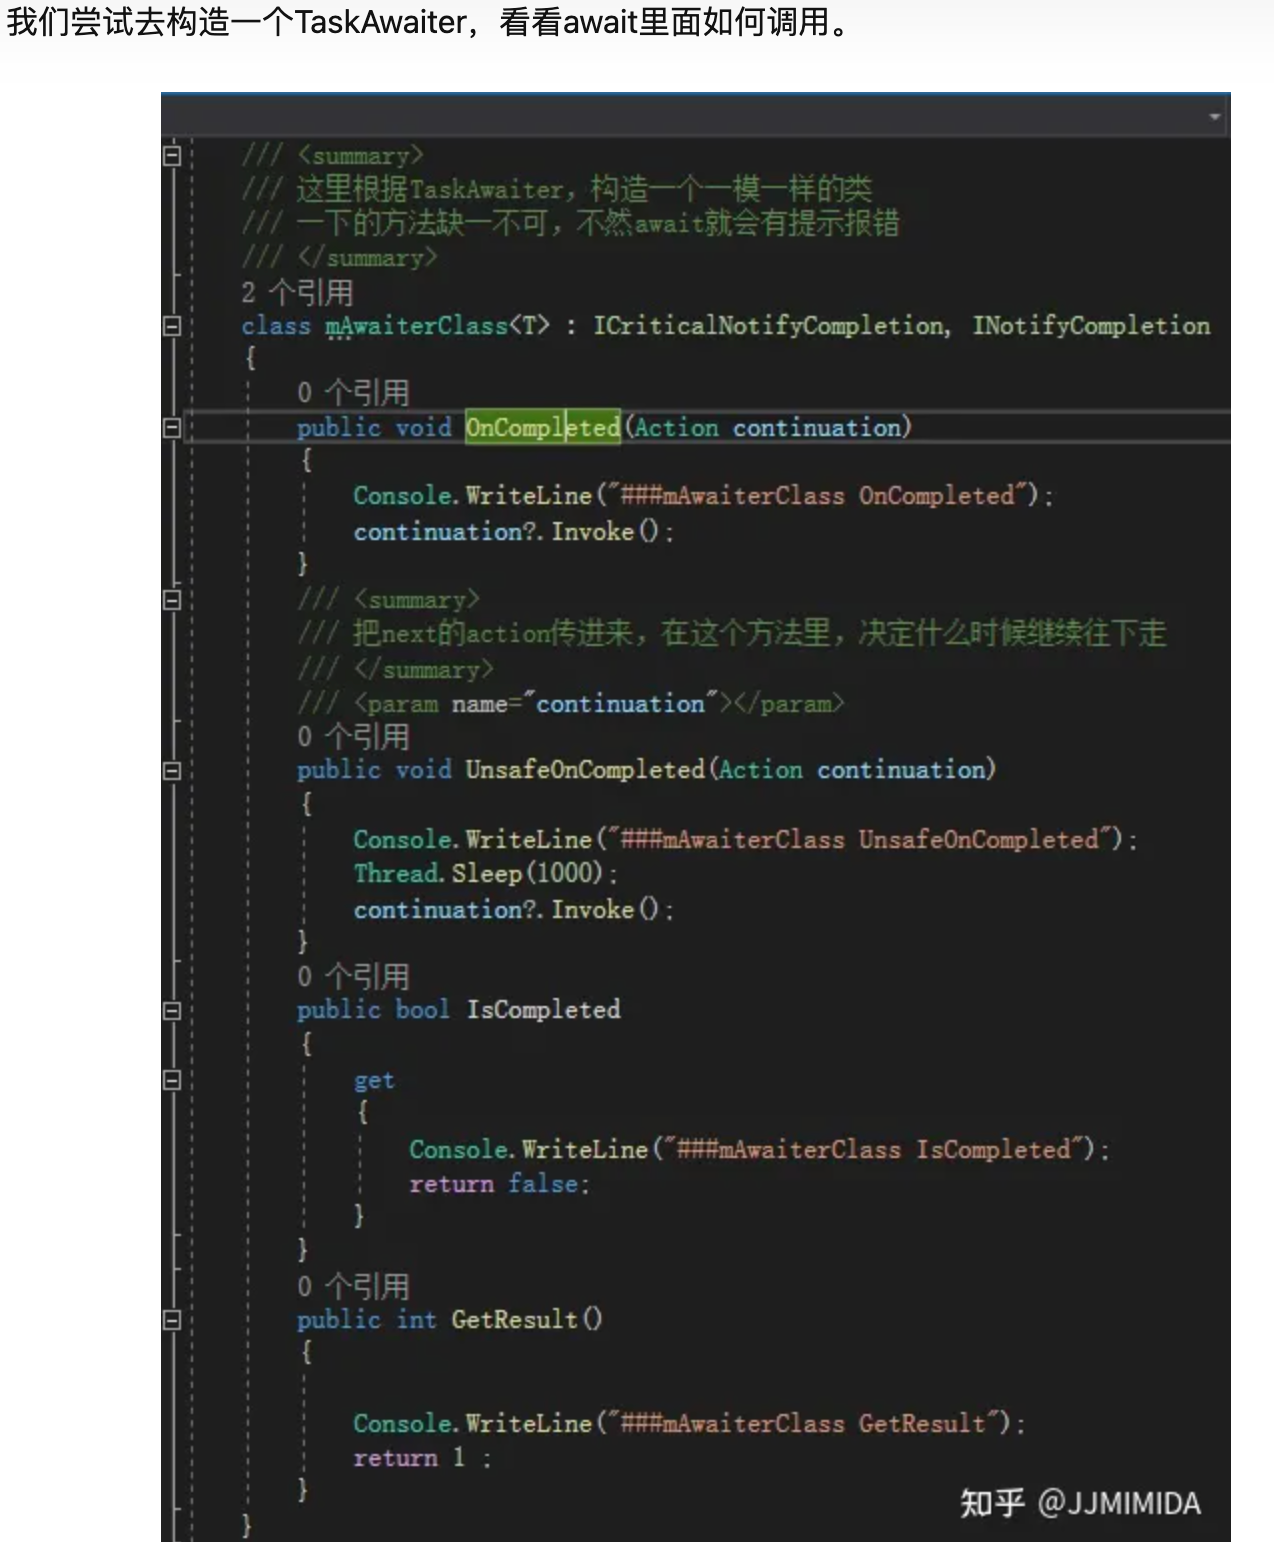
\includegraphics[width=.9\linewidth]{./pic/et3_20230609_105627.png}
\begin{itemize}
\item 它的测试用例是这么写的:注意它传入的参数类型是 int. 后面的编译码里,和它的讲解里会用到提到。
\end{itemize}

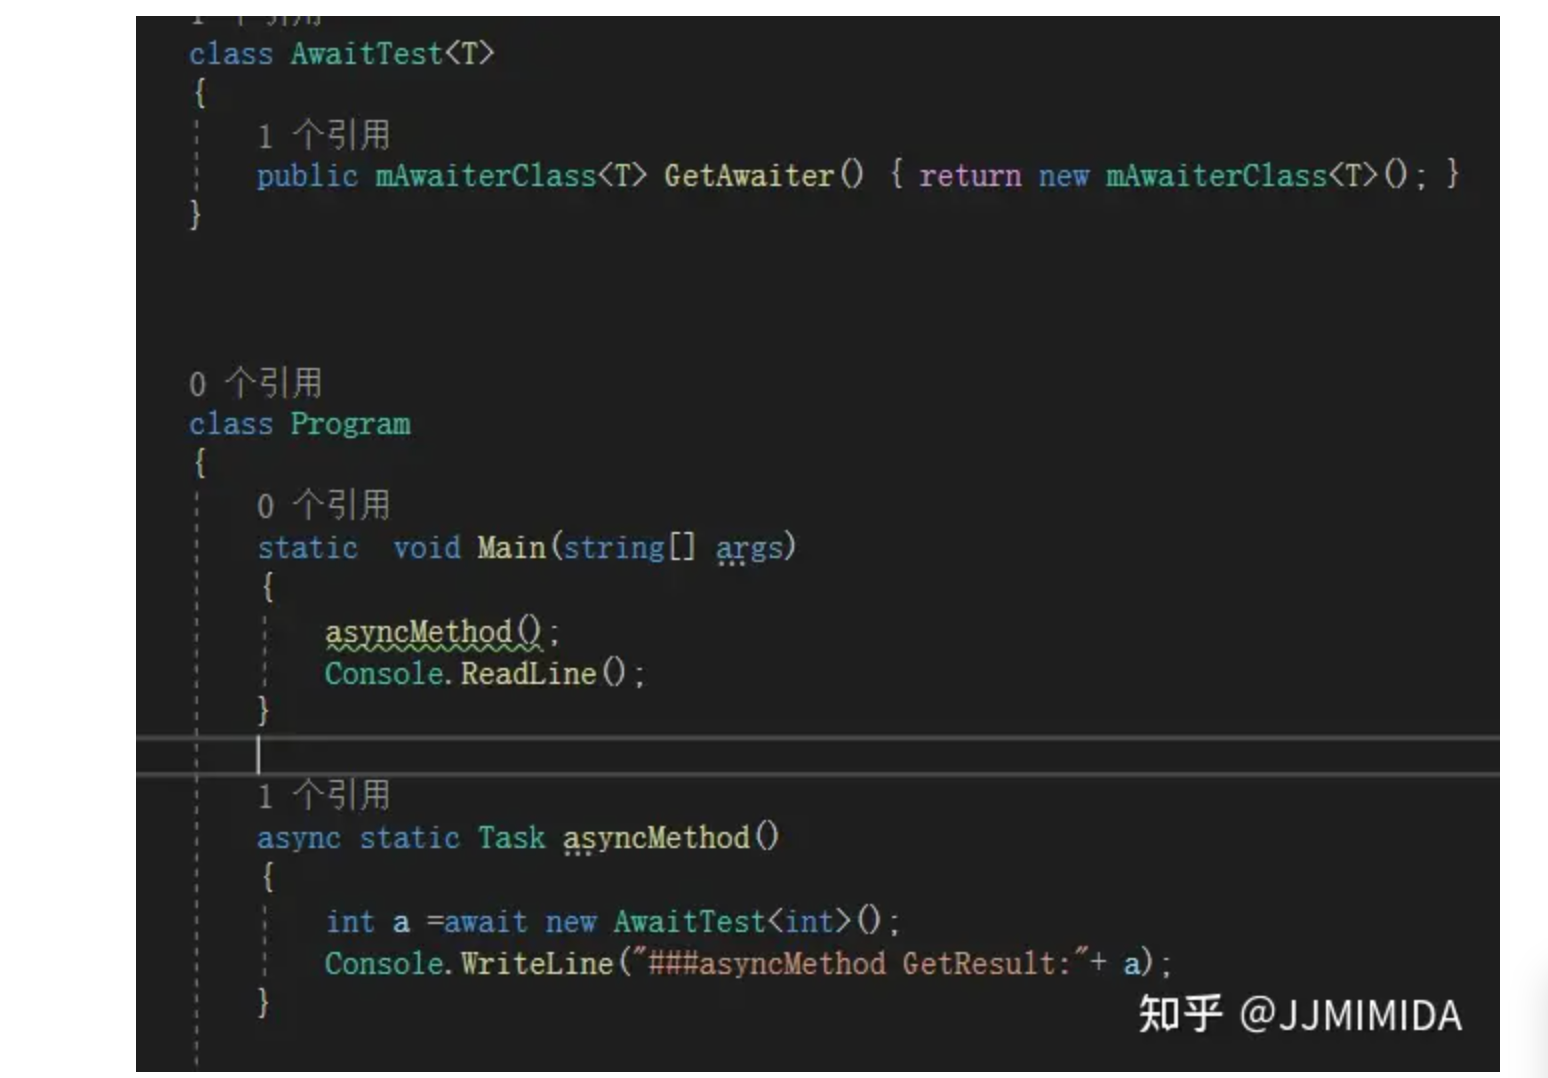
\includegraphics[width=.9\linewidth]{./pic/et3_20230609_105927.png}
\begin{itemize}
\item 看它编译出来的码(那堆编译出来的状态机的码),就是看不懂
\end{itemize}

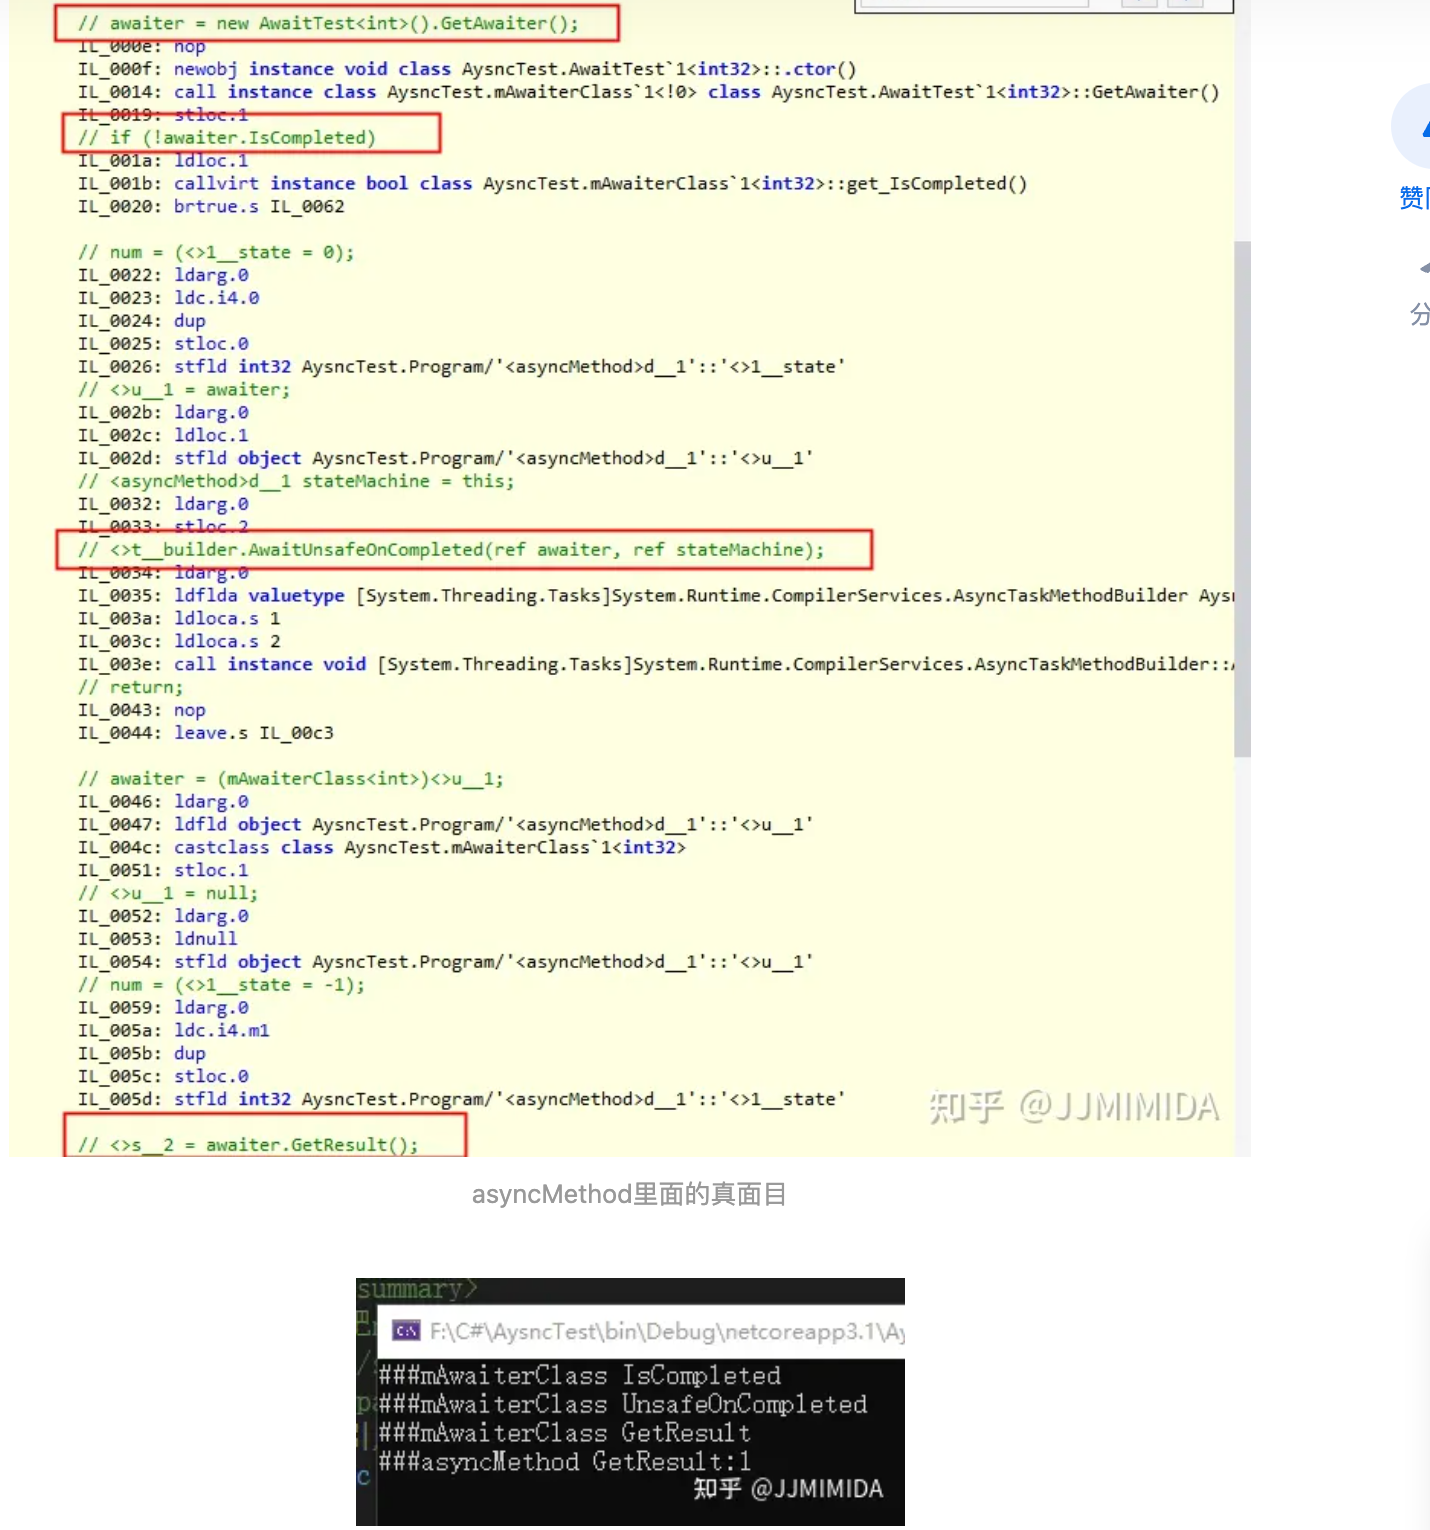
\includegraphics[width=.9\linewidth]{./pic/et3_20230609_112727.png}
\begin{itemize}
\item 结果分析: \textbf{【异步方法状态机,背后的执行顺序与逻辑:】}
\begin{itemize}
\item 先检查IsCompleted标志位,如果已经完成,则调用GetResult作为await的返回值返回。
\item 如果未完成,经过AsyncTaskMethodBuilder的AwaitUnsafeOnCompleted方法之后,最后进入UnsafeOnCompleted(nextAction),并且把完成后的下一步回调传进来。
\item 当我们获得nextAction之后,说明该调用由我们自己来控制,这里我在等待1s之后,执行nextAction(),下一步GetResult返回。
\end{itemize}
\item \textbf{【Async 关键字方法的编译原理:】}
\end{itemize}

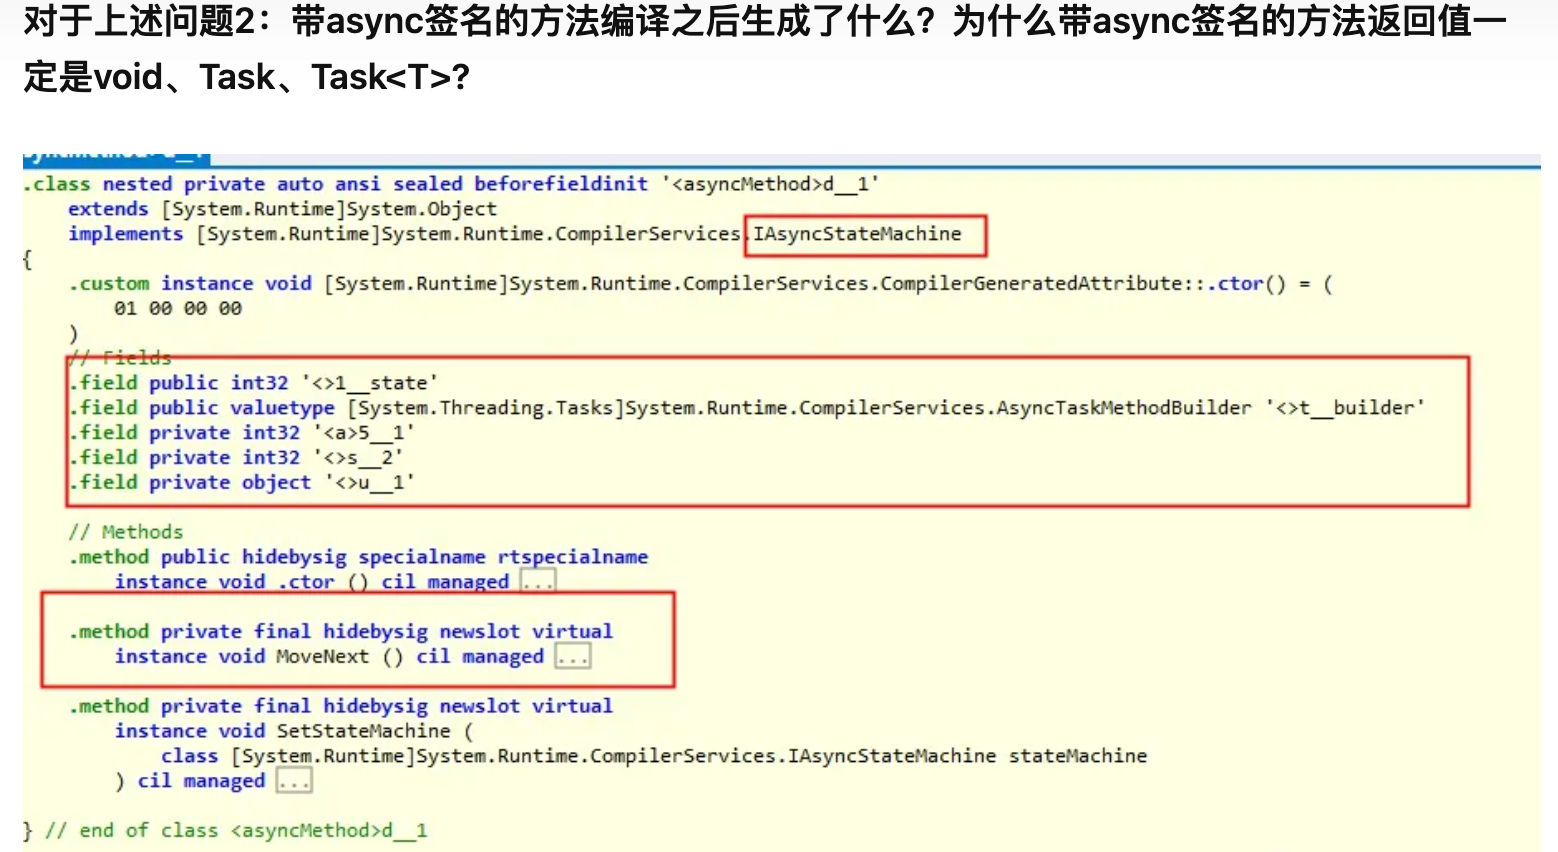
\includegraphics[width=.9\linewidth]{./pic/et3_20230609_110634.png}
\begin{itemize}
\item 这个 async 关键字所标记的异步方法,主要两个点儿: 
\begin{itemize}
\item 编译器,把这个异步方法,编译成了一个类 class <asyncMethod>d\_\_1;
\item 这个类 class, 它实现了 IAsyncStateMachine 接口,( \textbf{实现了这个接口,返回的是什么类型呢?} 这个要想明白?)
\item 这个类 class, 的内部,有几个成员变量 .field-sss.
\item 这个类 class, 的内部,有个特别重要的状态机执行函数 MoveNext() 来指挥指导,异步函数内不同节点如 await 节点等的执行逻辑。 \textbf{【这个类 class, 它实现了 IAsyncStateMachine 接口】}, 前面有列出 IAsyncStateMachine 接口定义的两个方法,所以实现实体类里也会有SetStateMachine() 方法的实现。
\item 上面的逻辑,其实是就是扫描异步方法内,不同的 await 调用,每到一个这个关键字申明的异步调用,就是切换一个状态(背后有可能是线程的切换, 不一定每个分支都用不同的线程,但线程的切换可能是,必要的时候需要切换的?)分段执行。
\end{itemize}
\item 网络上的分析者还给出了下机的截图:不是狠懂,这个截图是什么意思?因为不懂,要把编译码的方法名带上,方便以后再读和理解。
\end{itemize}

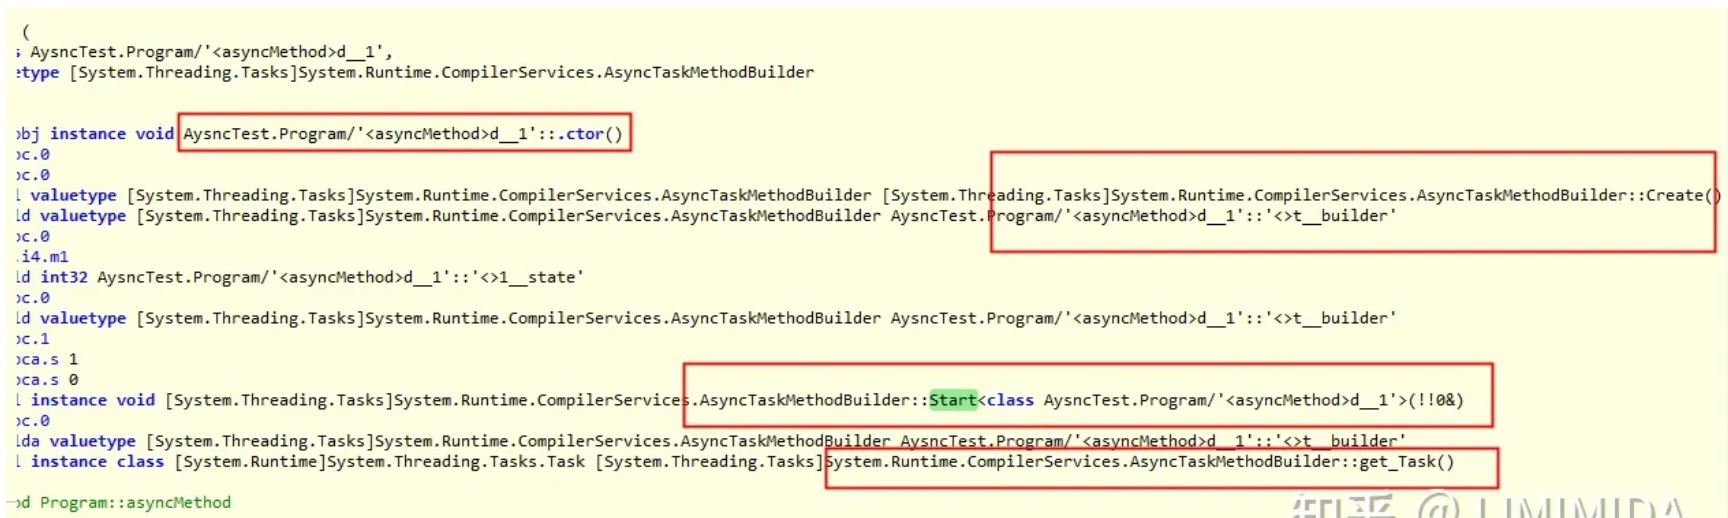
\includegraphics[width=.9\linewidth]{./pic/et3_20230609_112757.png}
\begin{itemize}
\item 上面的异步方法,所生成的异步状态机类 class 里,有几个主要的方法:
\begin{itemize}
\item 构造器方法 ctor():
\item Create() 方法:
\item Start() 方法:
\item get\_Task() 方法:
\end{itemize}
\item 可是上面的几个方法是谁,哪个接口定义的呢?
\item 网络上的分析者,对上面两个截图的分析如下: \textbf{【它讲解的这部分,我可能还是得自己编译一下,去具体看一下。】因为它的截图不完整,看不懂} 下面还有个别人总结的状态机套路,感觉说得更彻底透彻。
\begin{itemize}
\item 签名为async Task asyncMethod()的方法里,先创建一个继承自IAsyncStateMachine的asyncMethod类
\item 创建一个AsyncTaskMethodBuilder,然后赋值给Machine. (不知道,它这句,说的是哪里?第一个图的最后 SetStateMachine()?)
\item 初始化Machine的state = -1. (两个截图里看不见,找不到)
\item 调用AsyncTaskMethodBuilder.Start方法,start里面会进入Machine的moveNext()方法,详见问题1。
\item AsyncTaskMethodBuilder.get\_Task() 作为该方法的返回值返回。
\end{itemize}
\item 多线程问题: Task一定是多线程吗?
\begin{itemize}
\item 不一定,在上述例子中,我们定义的 async static Task<int> aa(),里面就是在同一个线程执行的。只有调用Task.Start 或者Task.Run 里面自动启用多线程的时候,才是多线程。
\end{itemize}
\item 看得另一个网页中的说法,因为感觉它也没有实现个什么公共定义约束的接口,理解得不够透彻。看下下面的:
\item await 必须配合 Task/ValueTask 才能用吗?当然不是。
\begin{itemize}
\item 在 C\# 中 \textbf{只要你的类中包含 GetAwaiter() 方法和 bool IsCompleted 属性,并且 GetAwaiter() 返回的东西包含一个 GetResult() 方法、一个 bool IsCompleted 属性和实现了 INotifyCompletion,那么这个类的对象就是可以 await 的} 。这里说得还是不清楚,不透彻,换一个表达得更清晰的说法如下:
\end{itemize}
\item 可以使用await的方法,返回值必须是 \textbf{awaitable对象} ,自定义awaitable对象比较麻烦,一个对象必须满足下列条件才行:
\begin{itemize}
\item 必须有一个 \textbf{GetAwaiter()} 方法,扩展方法或者实例方法都可以
\item GetAwaiter() 方法返回值必须是 \textbf{awaiter对象} 。一个对象要成为awaiter对象必须满足下列条件:
\begin{itemize}
\item 该对象 \textbf{实现接口 INotifyCompletion 或者ICriticalNotifyCompletion}
\item 必须有 \textbf{IsCompleted属性}
\item 必须有 \textbf{GetResult()方法} ,可以返回void或者其他返回值。
\end{itemize}
\end{itemize}
\item 比如下面的自定义类:把几个类的本质理解得再深一点儿了吗?【爱表哥,爱生活!!!任何时候,活宝妹就是一定要嫁给亲爱的表哥!!!】
\end{itemize}
\begin{minted}[fontsize=\scriptsize,linenos=false]{csharp}
public class MyTask<T> {
    public MyAwaiter<T> GetAwaiter() {// 必须提供的方法 
        return new MyAwaiter<T>();
    }
}
// 下面自定义的类 MyAwaiter<T=亲爱的表哥> 就是可以 await 的:
// 【任何时候,活宝妹就是一定要嫁给亲爱的表哥!!!活宝妹还没能嫁给亲爱的表哥,活宝妹就是永远守候在亲爱的表哥的身边!!!爱表哥,爱生活!!!】
public class MyAwaiter<T> : INotifyCompletion {// 必须实现的接口
    public bool IsCompleted { get; private set; }// 属性变量 
    public T GetResult() {// 必须要有的方法 
        throw new NotImplementedException();
    }
    public void OnCompleted(Action continuation) {
        throw new NotImplementedException();
    }
}
public class Program {
    static async Task Main(string[] args) {
        var obj = new MyTask<int>();
        await obj;
    }
}
\end{minted}
\begin{itemize}
\item \textbf{【状态机套路】:}
\item async关键字标记方法是一个异步方法,编译器通过这个标记 \textbf{【async关键字】} 去改造这个方法体为创建状态机的方法。await是关键字,是为了实现状态机中的一个状态, 每当有一个await,就会生成一个对应的状态。状态机就是根据这个状态,去一步步的调用异步委托,然后回调,包括状态机的解析。
\item (1).状态机的默认状态都是-1, 结束状态都是-2.
\item (2).每await一次就会产生一个 TaskAwaiter awaiter; 改变状态机的状态, 当有多个await的时候,每个await都会改变状态机的状态,比如 改为 0,1,2,3,4 等等, 分别表示代码中await xxx 这句话执行完成。
\item (3).状态机的执行套路:
\begin{itemize}
\item A. 首先创建一个 d\_num 的方法(这里说错了,应该是创建了一个类 class), xxx代表方法名,num可能是0,1,2,3等, \textbf{实现IAsyncStateMachine接口。}
\item B. 在MoveNext()方法中, 源代码中每个 await xxxx 都会对应生成是一个 TaskAwaiter awaiter,然后 xxxx.GetAwaiter()
\item C. 判断状态机是否执行完if (!awaiter.IsCompleted),
\begin{itemize}
\item 没有执行完的话走 <>t\_\_builder.AwaitUnsafeOnCompleted(ref awaiter, ref stateMachine); 代表释放当前线程
\item 执行完后走,<>s\_\_1 = awaiter.GetResult(); 拿到返回值,继续走后面的代码。
\end{itemize}
\end{itemize}
\item (此处写的比较抽象,看下面3 结合代码编译再分析)
\item 感觉今天读这个状态机:\url{https://linuxcpp.0voice.com/?id=1380} 终于有点儿开窃了!!【爱表哥,爱生活!!!任何时候,活宝妹就是一定要嫁给亲爱的表哥!!!爱表哥,爱生活!!!】
\end{itemize}
\subsection{如果方法声明为 async,那么可以直接 return 具体的值,不再用创建Task,由编译器创建 Task:}
\label{sec-4-2}
\begin{minted}[fontsize=\scriptsize,linenos=false]{csharp}
// 只要标记了async 就会被编译成状态机
// 如果方法声明为 async,那么可以直接 return 具体的值,不再用创建Task,由编译器创建 Task: 
  public static async Task<int> F2Async() {
      return 2;
  }
\end{minted}
\begin{itemize}
\item F2Async:只加了async,会生成状态机,但由于没有加await所以不会涉及到中间状态的变化,从-1默认状态 变为 结束的-2状态。
\end{itemize}
\begin{itemize}
\item F3Async:既有async也有await (await只有1个),该方法是使用了Task.Run,我们把它归为计算型的异步方法。
\item 亲爱的表哥,活宝妹今天终于把这个看得稍微有点儿懂了,希望能够赶快从这个ETTask 模块 move-forward. 任何时候,活宝妹就是一定要嫁给亲爱的表哥!!!活宝妹还没能嫁给亲爱的表哥,活宝妹就是永远守候在亲爱的表哥的身边!!!爱表哥,爱生活!!!
\end{itemize}


\section{现在的修改内容:【任何时候,活宝妹就是一定要嫁给亲爱的表哥!!!爱表哥,爱生活!!!】几大版块}
\label{sec-5}
\subsection{热更新层的生成系}
\label{sec-5-1}
\begin{itemize}
\item \textbf{【热更新层的生成系】} :下午家里试着把Component 组件再添加回去试试看 \textbf{【不能再添加Component 组件。ET7 框架重构了,小单元也走热更新,在热更新层有天文小行星的生成系。可以参照 ET.pdf 里的服务端 PlayerSystem 来作例子】} ?上午把项目设计的思路,源项目的破源码再读一读理一理,是希望游戏逻辑与游戏界面能够快速开发、项目进展往后移的。
\begin{itemize}
\item \textbf{【热更新层的生成系】} :不少组件,我急着添加热更新层的生成系的时候,可能忽略了某些必要、不必要的Awake() 系统。运行时如果抛错,可以补上必要的Awake() 等必要的框架系统方法。比如:LandlordsGateSessionKeyComponentSystem, 它需要Awake() 系统吗?再列一个报错的例子:C2G\_LoginGate\_ReqHandler. 【改法】:如果不强改成是单个游戏逻辑,ET 框架里有这个逻辑处理,可以去参考原框架的写法与生成系是如何自动绑定的。
\item User.cs 客户端的话,不知道要不要修改。晚点儿的时候留意一下。
\item Gamer.cs 客户端保留了 Dispose
\end{itemize}
\item \textbf{【IMHandler】} :在 ET7 的框架里,Handle() 方法的定义,主要是Actor 消息机制大概又重构得更为自动化一点儿,当有分门别类的ActorMessageHandler 标签系实体类,大概ET7 框架里只需要调用接口的申明方法就可以了?总之,就是Handle() Run() 两大类方法的方法定义发生了变化
\begin{itemize}
\item 在IMHandler 的两个抽象实现类的封装里,ET7 构架重构后,各种服需要自定义的服务器处理逻辑被要求实现在 Run() 方法里;而抽象类定义的Handle() 方法里,自动封装实现了带回复消息的请求消息的自动回复(通过抽象类里实现方法调用 Session.Send(XXX))。这个对需要返回消息的请求消息的自动回复的封装,有利有不利
\begin{itemize}
\item 利是:当顺序不重要,可以自动回复时,由框架的底层帮实现自动回复,方便
\item 不利是:当顺序变得重要,当回复消息后,某个某些服还有其它逻辑需要服务器来处理,这个框架底层的自动封装就会成为一个 blocker, 需要自己想办法去解决这些特殊服,要如何实现必要情况下的,先回复消息,再处理服务器端的其它逻辑。【这片儿哪里作过这个笔记,有个细节的服务器端的实现处理逻辑,顺序重要】
\end{itemize}
\item AMRpcHandler 的实体实现类,我可能还需要再多找几个出来看下
\item 今天下午弄这些IMHandler 以及两个抽象实现类,和它们服务端的消息处理器类,编译氏错误一堆,感觉昨天下午基本都消干净了。接着崩出来的 214 个框架里的其它错误都能一一解决,昨天晚上消掉了大概 100 个左右的编译错误。它们是框架里的细节,是帮助活宝妹理解这个框架的方方面面点点滴滴的必经步骤。活宝妹不怕它们,也没什么可怕的。。。【爱表哥,爱生活!!!任何时候,活宝妹就是一定要嫁给亲爱的表哥!!爱表哥,爱生活!!!】
\end{itemize}
\end{itemize}
\subsection{内网消息等网络相关:请求消息的发送方法等。狠多编译错误,要一点儿一点儿把他们都改掉}
\label{sec-5-2}
\begin{itemize}
\item \textbf{【内网消息等网络相关:请求消息的发送方法等】}: \textbf{在构架里是怎么写的,有几种请求消息的发送方式?}
\item \textbf{明天上午把这块看完,等着我改的编译错误包括} :参考的斗地方游戏里,各种服处理返回消息的逻辑。
\begin{itemize}
\item 因为先前手动发送每个返回消息,我需要将这部分一批消息处理器改为,先试着适配 ET7 框架的重构与底层再封装。
\item 等改过了,真正明白理解了自己重构游戏的需求,再来看去看ET7 框架我要怎么改它现存封装,才能适配自己游戏的需求!!例子:MatchComponentSystem 里的JoinRoom 方法等相关逻辑。
\item 【下午还没有改到这里来。先从简单的改起,因为一个热键的优化,感觉VS 好用一点儿了。先能改多少改多少,再按模块来改像消掉所有的ETTask 相关一样把一个模块的所有的编译错误全部改完!!!】
\end{itemize}
\item 去看上面列过的那个例子MatchComponentSystem, 参考项目里的各种服的消息处理,怎么适配成ET7 重构后的不用手动发返回消息(发送过程封装在框架底层),和记录可能存在的问题(某些服的逻辑,返回消息的发送时间与其它必要逻辑,顺序变得重要的时候,记下来,晚点儿会再重构ET7 框架适配游戏需求)
\end{itemize}
\subsubsection{修改下面的ActorMessageSenderComponent 因为功能模块逻辑重构,而带来的一堆编译错误。}
\label{sec-5-2-1}
\begin{itemize}
\item 修改方法过程步骤:去框架里搜索,其它任何地方发送消息的例子,看 \textbf{【重构后的框架是如何发送消息的, Call() Send() 方法的调用等】} 这个明天上午一定看,因为不懂,不会改怎么发送消息的()
\item 然后参照例子,把客户端和必要的小服里,所有需要发送消息的地方,改成上面看到总结的发送方法里。
\end{itemize}

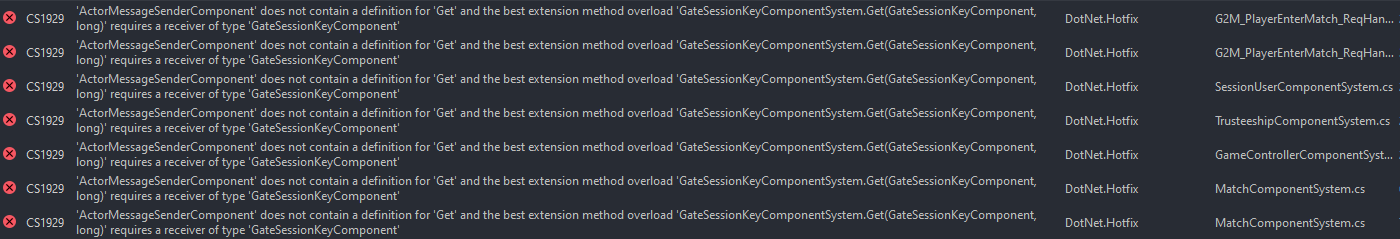
\includegraphics[width=.9\linewidth]{./pic/et4_20230616_160327.png}

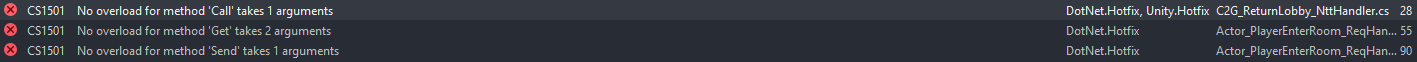
\includegraphics[width=.9\linewidth]{./pic/et4_20230616_165027.png}
\begin{itemize}
\item 今天上午就先看这个。要把发送消息弄明白了,要不然下午还是不会改。下午改到5pm 左右再出发,天气热,出去早了会被晒黑。亲爱的表哥的活宝妹现在狠漂亮,肝肾功能好了,皮肤白白亮亮,可不要再轻易被晒丑了!!!
\item 【地图服Unit 相关】:先前所有接触到这个框架,都只看了个头,就是只限于能够任何客户端连接到服务端能够注册登录的程度,后面的其它服、框架逻辑全都还不曾看。所以今天上午扫一眼地图服相关,是糊的。要把这些前前后后相关的原理总弄懂了。
\item 去框架里搜发送的调用方法,可能现在 Mac 系统里有一点儿障碍的,就是VSC 不报错,不知道搜出来的是对的,还是错的。但是几种不同的方法,先总结在这里,对照运行时的报错一一改过来。必须把这块儿弄明白了。【爱表哥,爱生活!!!任何时候,活宝妹就是一定要嫁给亲爱的表哥!!爱表哥,爱生活!!!】
\item 【拿到Session 会话框,调用其Send() 方法】:例子 PingComponentAwakeSystem 里的 PingAsync() 方法。它是一个心跳包。这个心跳包就是一Awake() 醒来,全生职责就是周期性给服务器发消息
\item 然后参照例子,把客户端和必要的小服里,所有需要发送消息的地方,改成上面看到总结的发送方法里。
\item 框架里,各种不同场景下发送消息的方法: \textbf{【今天下午有运行环境,三个小时,希望把这个模块总结完,几个相关的编译错误改完】}
\item 【场景里拿到SessionComponent】,调用会话框的发送方法Send()
\begin{minted}[fontsize=\scriptsize,linenos=false]{csharp}
robotScene.GetComponent<Client.SessionComponent>().Session.Send(new C2M_TestRobotCase2() {N = robotScene.Zone});

// 也可以借助UnitGateComponent 拿到它的成员变量 GateSessionActorId, 用这个可以重构后发消息
ActorMessageSenderComponent.Instance.Send(u.Unit.GetComponent<UnitGateComponent>().GateSessionActorId, message);
\end{minted}
\item 【活宝妹任何时候就是一定要嫁给亲爱的表哥!!!】迷迷糊糊地把一个模块改完了,可是感觉那个改掉的模块,像是还没能理解透彻。明天上午会再看一下。【爱表哥,爱生活!!!任何时候,亲爱的表哥的活宝妹,就是一定要嫁给亲爱的表哥!!爱表哥,爱生活!!!】70 Compile Errors 还没有改完,涉及功能模块人接入与整合。会明天上午看过读一下相关模块的源码后再试着改。【活宝妹就是一定要嫁给亲爱的表哥!!!爱表哥,爱生活!!!】
\end{itemize}
\subsubsection{【ActorMessageSenderComponent】:这个类狠重要、狠重要,现在是活宝妹理解网络模块的核心。爱表哥,爱生活!!!}
\label{sec-5-2-2}
\begin{itemize}
\item 得去想:ActorMessageSenderComponent, 是只能用来处理跨进程消息的吗?普通消息的发送是如何处理的?该弄明白,它的适用范围,适用哪些情境上下文
\item \textbf{【ActorMessageSenderComponent】} :因为ET7 这个模块的重构。不再需要每个返回消息手动去拿消息发送器,交由框架底部去处理。
\item 不懂的是,如何重构,消除参考项目里各种服的消息处理里,怎么适配成ET7, 不用去拿消息发送器,只把返回消息结果写好,或是发送(请求)消息时,如何发送?
\item 不同于昨天上午看过的,NetInnerComponentOnReadEvent 是对上层读到消息后的处理,就是消息已经准备好了,甚至已经通过某种逻辑代理,到达和触发了NetInnerComponentOnRead 事件了(这个事件是怎么触发的?大概是,每个进程会有一个内网组件NetInnerComponent. 当内网组件读到消息会触发。读到消息,包括本进程消息,也就包括,由其它进程发回来的返回消息。这个,可能更底层Session 发回来跨进程消息的地方?改天去捡)。现在要去理解的是,比如发送一条请求消息,创建一个请求消息实例后,如果运动可以走到上面的触发读到消息事件?就是消息流程的前半部分。NetInnerComponentSystem.cs 的读到消息事件,要再往前看一点儿。
\item 把消息的处理流程几个重要的方法 \textbf{【ActorMessageSenderComponentSystem Send() Call() 等】} ,这里再梳理一遍:
\end{itemize}
\begin{enumerate}
\item ActorMessageSenderComponentSystem Send():
\label{sec-5-2-2-1}
\begin{itemize}
\item \textbf{【ActorMessageSenderComponentSystem Send()】} 发的是普通消息(不是不需要回复消息,是任何消息,都走这一步,因为是最基的基类接口)
\begin{itemize}
\item 【同一进程消息】:不走网络层,直接交由本【进程?】的消息处理器处理。就是(ActorMessageSenderComponentSystem Send()里)判断如果是同一进程,它会调用内网组件处理消息:NetInnerComponent.Instance.HandleMessage(actorId, message); 【注意这里是一个进程内网组件消息的一个来源:本进程消息。它同样接收和读来自其它进程的消息,跨进程消息】。而内网组件的这个HandleMessage() 静态方法,就发发布内网组件读到消息事件;内网组件读到消息事件的发布,会触发调用 NetInnerComponentOnReadEvent 借助 ActorHandleHelper 来处理内网消息。后面的就是昨天上午读到的部分。这里的疑问就是:谁,哪里调用发送组件的Send() 发送事件?
\item 【不是同一进程消息】:就通过内网组件,去拿同那个收消息进程的会话框,通过会话框走Session 流程发跨进程消息。就是走网络层。
\end{itemize}
\end{itemize}
\item ActorMessageSenderComponentSystem Call()
\label{sec-5-2-2-2}
\begin{itemize}
\item \textbf{【ActorMessageSenderComponentSystem Call()】} 发的是要求返回结果的消息:返回 ETTask<IActorResponse>
\begin{itemize}
\item 注意 \textbf{【跨进程消息的回复细节里】} ,看见IRpcResponse 实例创建好,结果写好,同步到异步任务ETTask 里,总容易忘记ETTask 的异步任务运行结束(如果不是抛异常), \textbf{跨进程消息是如何回到消息的发送进程的?} 是AMRpcHandler 抽象类里,异步等待实体实现类里的具体实现逻辑Run() 异步方法执行结束,也就是等待各种消息处理服处理好、写好异步返回消息IRpcResponse, 同步到异步任务ETTask. AMRpcHandler 抽象类里等异步方法执行完成,抽象类里作了封装,把返回消息通过进程间通信会话框,把返回消息发回去的。
\item 这里看见,这个消息发送器底层逻辑说,如果是我自己进程要发消息,就封装消息发送者 rpcId 是自已的 rpcId. 然后调用自组件Call() 发送消息。后面的几个方法,大概就是跨进程消息的发送与回复。
\end{itemize}
\end{itemize}
\end{enumerate}
\subsection{框架里现存的错误:载图,明天上午把功能模块一一看一遍,现在不知道怎么改了,要再看再学习了才会改}
\label{sec-5-3}
\begin{itemize}
\item 现框架里不存在的,需要整合进来的模块版块:
\end{itemize}

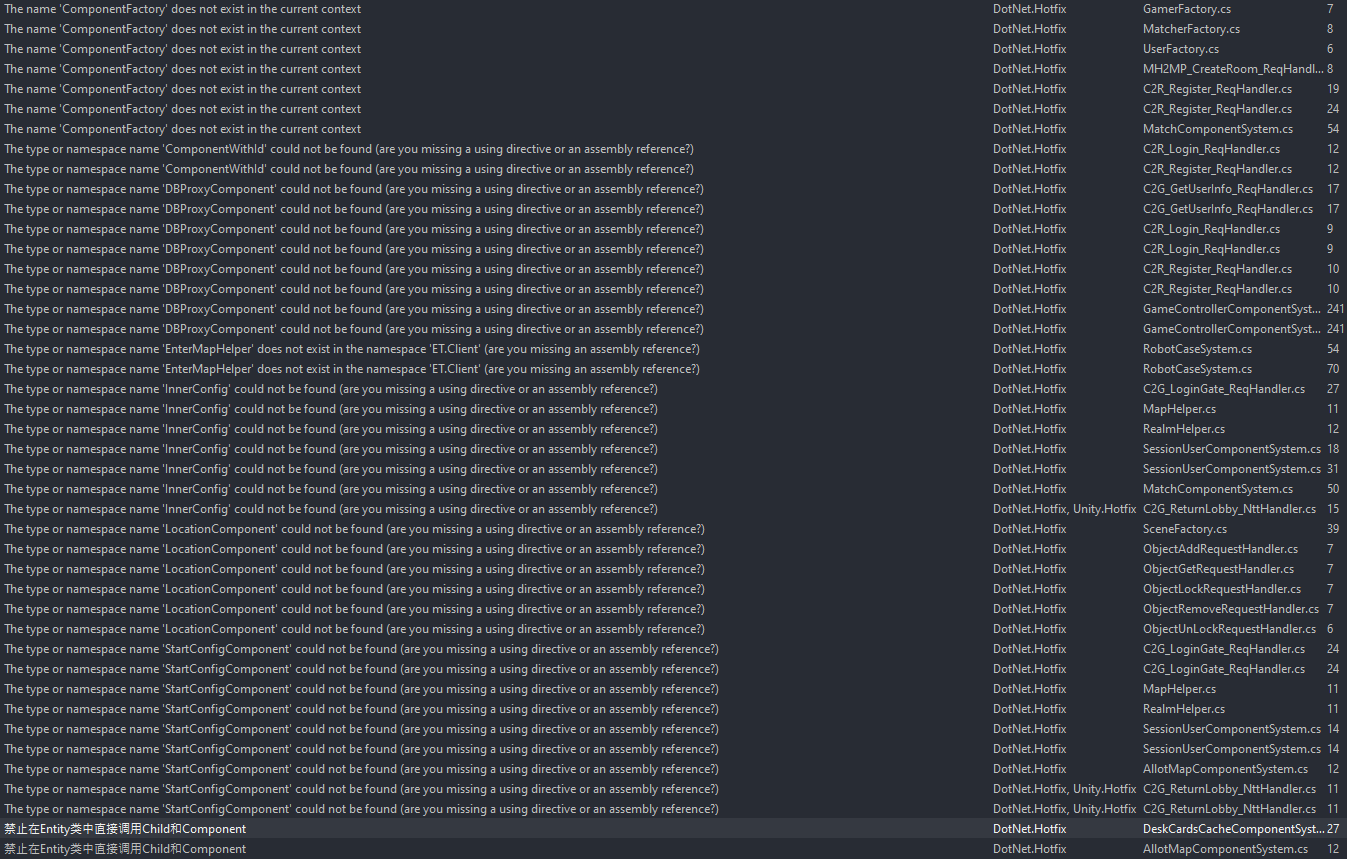
\includegraphics[width=.9\linewidth]{./pic/et4_20230616_165750.png}
\begin{itemize}
\item 【ComponentFactory:】重构了的框架里,这个工厂类是被折解到各自小部件的生产工厂里去了,就是一个框架底层封装的工厂类,拆解到 100 个不同的小部件里。所以我必须得要每个使用的小部件里,它的生产工厂里去再调用相应的逻辑。【可以找个例子出来看一下】
\begin{itemize}
\item Entity 类里面有,组件里添加一个新 new 出来的成员的办法。模仿Player 的使用例子。这里的使用方法是:去拿它的管理组件的实例索引,用管理组件来生成各个元件
\item 同样套用的话,GamerComponent 是房间组件的子组件,拿到这个组件后来创建
\end{itemize}
\item \textbf{【ComponentFactory.CreateWithId:】} 重构了的框架里,这个工厂类是被折解到各自小部分的生产工厂里去了,就是一个框架底层封装的工厂类,拆解到 100 个不同的小部件里。所以我必须得要每个使用的小部件里,它的生产工厂里去再调用相应的逻辑。【可以找个例子出来看一下】新框架里,上次不是找到过:先去拿管理器组件,再用管理器组件,通过调用基类Entity 里的方法,来创建小部件的实例?可以再找个例子看一下
\item 上午把【数据库模块的接入】、【InnerConfig】【StartConfigComponent】【LocationComponent】等相关模块:读下源码,理解透彻,必要的情况下下午家里接入并测试
\begin{itemize}
\item \textbf{【数据库模块:】} 现框架中被砍得几乎不剩下什么,如果弄不懂,可以与参考项目斗地主中的数据库模块作对照来理解,和添加必要的类等。
\item 如果这一块儿,这会儿还没什么头绪,就先看看别的呀
\end{itemize}
\item 把IMHandler 接口,以及它的两个抽象实现类、相关模块的部分理解透彻
\item 上午就是看那几个框架里还不熟悉的模块,能看懂哪些,就先看先事理哪些。
\item 先看只看了一半的,比如什么IMHandler 接口的实现类等,如果今天上午有机会,也可以看一下
\item 其它几个杂项错误:
\end{itemize}

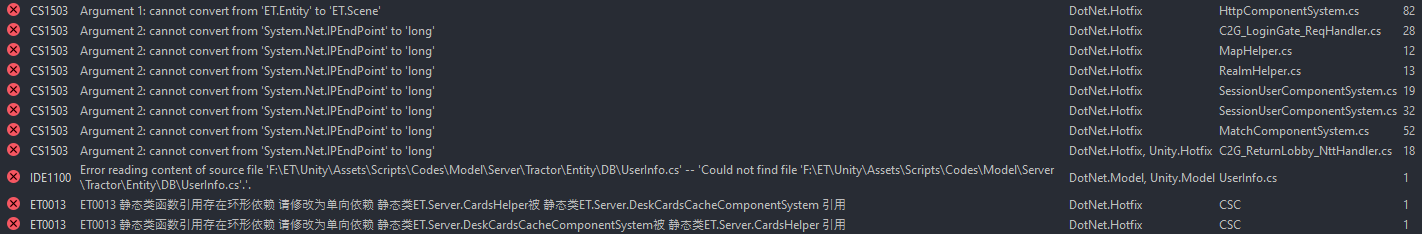
\includegraphics[width=.9\linewidth]{./pic/et4_20230616_165627.png}
\begin{itemize}
\item 下面是已经改好了的:还是先放着,备查
\end{itemize}

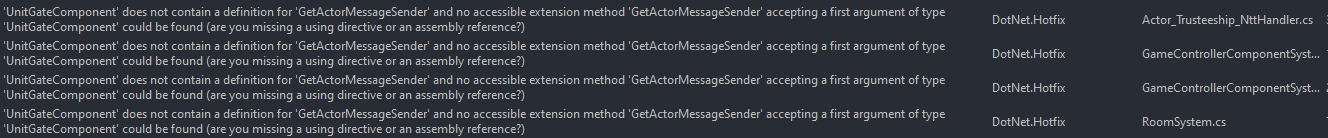
\includegraphics[width=.9\linewidth]{./pic/et4_20230616_162711.png}
\begin{itemize}
\item 【UnitGateComponent]: 怎么才能成为多个不同组件的组成部分?
\end{itemize}

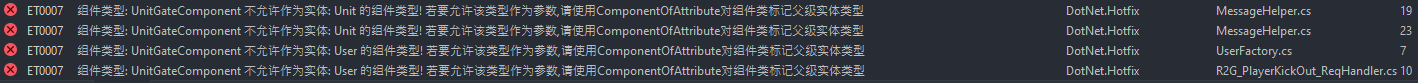
\includegraphics[width=.9\linewidth]{./pic/et4_20230616_165317.png}
\begin{itemize}
\item 【解决办法】:去查框架里的源代码,写得极其清楚:
\begin{minted}[fontsize=\scriptsize,linenos=false]{csharp}
// 组件类父级实体类型约束
// 父级实体类型唯一的 标记指定父级实体类型【ComponentOf(typeof(parentType)】
// 不唯一则标记【ComponentOf]
[AttributeUsage(AttributeTargets.Class)]
public class ComponentOfAttribute : Attribute {
    public Type Type;
    public ComponentOfAttribute(Type type = null) {
        this.Type = type;
    }
}
\end{minted}
\begin{itemize}
\item 所以上面的解决办法就是:不要标记 typeof 参数就可以了呀,它就可以成为多个不同组件的子元件部件了呀。。。是这样的
\end{itemize}
\begin{minted}[fontsize=\scriptsize,linenos=false]{csharp}
[ComponentOf] 
public class UnitGateComponent : Entity, IAwake<long>, ITransfer, ISerializeToEntity { // 不知道这里为什么会受到限制,这里再改一下
    public long GateSessionActorId { get; set; }
    // 想一下,下面的变更还需要吗?要不要,是看框架里有没有什么,自动上线自动下线处理之类的,相关的?
    public bool IsDisconnect;
}
\end{minted}
\end{itemize}
\subsection{先前列的相对杂一点儿}
\label{sec-5-4}
\begin{itemize}
\item 【问题】:上次那个ET-EUI 框架的时候,曾经出现过 opcode 不对应,也就是说,我现在生成的进程间消息,有可能还是会存在服务器码与客户端码不对应,这个完备的框架,这次应该不至于吧?
\item 【UIType】部分类:这个类出现在了三四个不同的程序域,现在重构了,好像添加得不对。要再修改
\item \textbf{【ET7 框架】} 没有处理的逻辑是: \textbf{【ET7 框架里数据库的接入】}
\item \textbf{【UILobbyComponent 可以测试】} :这个大厅组件,Unity 里预设简单,可以试运行一下,看是否完全消除这个UI 组件的报错,这个屏的控件能否显示出来?还是错出得早,这个屏就出不来已经报错了?
\begin{itemize}
\item 【客户端】的逻辑是处理好了,编译全过后可以测试
\item 【服务端】:处理用户请求匹配房间的逻辑,仍在处理: \textbf{C2G\_StartMatch\_ReqHandler}.
\end{itemize}
\item \textbf{【TractorRoomComponent】} :因为是多组件嵌套,可以合并多组件为同一个组件;另早上看得一知半解的一个【ChildOf】标签,可以帮助组件套用吗?再找找理解消化一下
\item 【房间组件】:几个现存的 working-on 的问题:
\begin{itemize}
\item 多组件嵌套:手工合并为一个组件。彻底理解确认后,会合并
\item 【服务端】:处理用户请求匹配房间的逻辑. 这里的编译错误终于改完。到时就看运行时错误了。
\begin{itemize}
\item 【数据库模块的整合】:网关服在转发请求匹配时,验证会话框有效后,验证用户身份时,需要去【用户数据库】拿用户数据。ET7 留了个DBManagerComponent, 还没能整合出这个模块
\end{itemize}
-【参考来源 \textbf{C2R\_LoginHandler} 】:Realm 处理客户端的登录请求的服务端逻辑。这里看见,它随机分配一个网关服。也就是,我(原本本质上也是随机分配)一个匹配服给用。可以依照这里的例子来改写。
\end{itemize}
\item 【匹配服地址】网关服的处理逻辑里,验证完用户合格后,为代为转发消息到匹配服,但需要拿匹配服的地址。ET7 重构里,还没能改出这部分。服务器系统配置初始化时,可以链表管理各小构匹配服,再去拿相关匹配服的地址。ET7 框架里的路由器系统,自己还没有弄懂。
\item \textbf{【ET7 IMHandler 对回复消息的写封装, 与自动回复消息的封装】} :可能无法处理游戏过程中的某些逻辑。就是涉及到一定顺序,尤其需要先回复消息的处理服处理逻辑。举例:C2G\_StartMatch\_ReqHandler. 所以,这里要自己好好想透彻一点儿。要如何改,才能适配自己游戏的需求。
\item \textbf{【 ComponentFactory:】} ET7 里重构,被分布到各种不同的组件里去了。想复制个文件过来,把与之相关的全部消掉,但因为大规模重构,复制了文件也没用。总之ET7 就是感觉什么乱七八糟的,感觉他们大规模糊乱重构的目的就是故意挫败人。可是这个世界上就偏偏存在亲爱的表哥的活宝妹这样的不服的!!!爱表哥,爱生活!!!任何时候,活宝妹就是一定要嫁给亲爱的表哥!!!爱表哥,爱生活!!!

\item \textbf{【PlayerComponent 类重复】} : 狠奇怪:删除了说找不到类,不删除说重复了,感觉台式机应用有延迟?反应狠慢。。。。。文件嵌套想要显示所有嵌套文件的时候,要狠久狠久重启好几次才反应得过来
\begin{itemize}
\item 原本有两个类都是如上面这个类这样,但有时候台式机反应稍快一点儿,就是一个类找不到出现上面的情况。破电脑的延迟反应,弄得我都要怀疑VS 应用被别人操控了。。。
\item 【爱表哥,爱生活!!!任何时候,活宝妹就是一定要嫁给亲爱的表哥!!!爱表哥,爱生活!!!】
\end{itemize}
\item 把还没有用到,但是报错了的几个类删掉:比如记一下: SessionInfoComponent,
\begin{itemize}
\item 还剩最后 26 个最挑战活宝妹的编译错误,今天傍晚会家里改会儿,集中问题明天上午希望能够看懂。【爱表哥,爱生活!!!任何时候,活宝妹就是一定要嫁给亲爱的表哥!!】
\end{itemize}
\end{itemize}

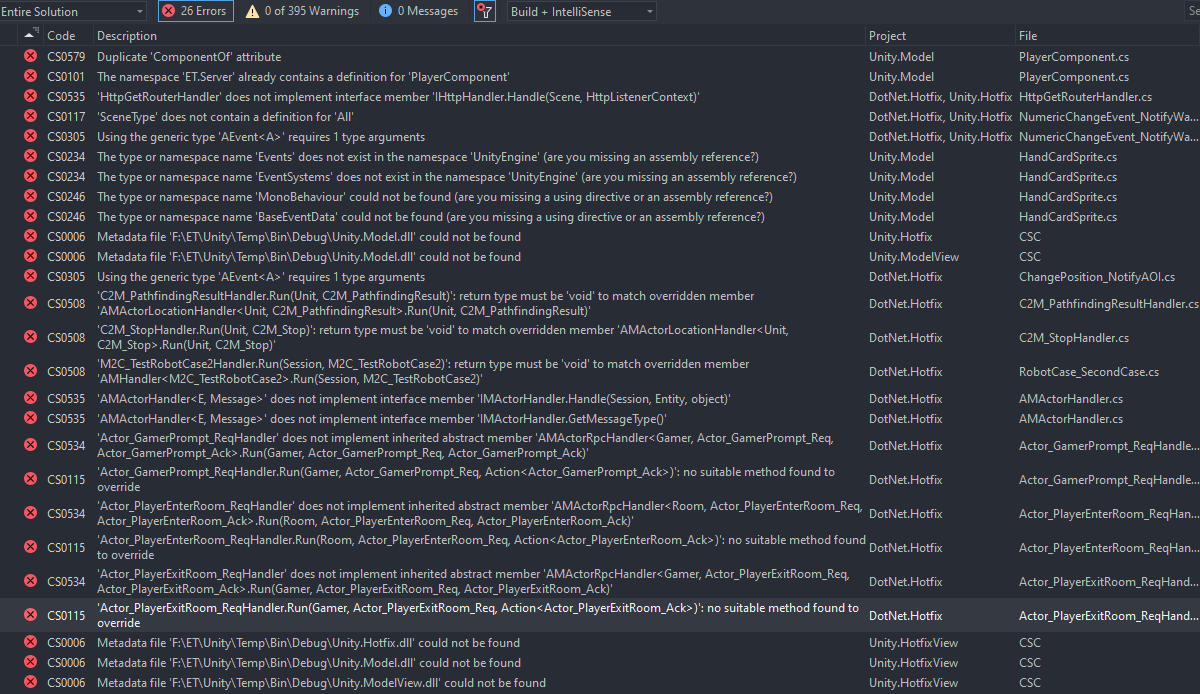
\includegraphics[width=.9\linewidth]{./pic/et4_20230604_162732.png}
\begin{itemize}
\item 把Root 根场景以及启动时添加的组件大致看了一遍。想把上面的消息处理器再系统化地看一遍,理解一下,总改不到这个模块相关的编译错误。
\item \textbf{【ETTask ETVoid 是必须弄懂的】} ;看两个小时,像昨天晚上一样真正投入进去看。我相信自己看得懂,弄得透,只是需要投入一点儿时间。
\begin{itemize}
\item 感觉前一个周左右的时间,倍受睡眠困扰。活宝妹做梦也不会想到,昨天的自己会困成那个样子(感觉开1 小时的车极度困难,太容易睡着。。)。。现在试着一再调整状态,少喝咖啡多运动,最重要的,仍是把学习的状态调整出来调整回来。至少学到活宝妹可以嫁给亲爱的表哥的这一天!!!
\item 这个异步的原理,感觉是弄明白了,今天上午又看了一遍看了会儿。下午去改那些 IMHandler, 希望今天下午能够改彻底。就是真正弄明白了去改(现在的问题就是,几个IMHandler 的实体实现类,改天这个顾不了那个,没弄明白,接口方法怎么申明定义,才能兼顾所有实例类消息处理器?),不是只改掉了当前的编译错误,等真正运行的时候,一个个运行错误或是异常往外冒!!!今天脑袋还算清醒,下午好好弄弄这个
\end{itemize}
\item 【爱表哥,爱生活!!!任何时候,亲爱的表哥的活宝妹,都是一定要嫁给亲爱的表哥的!!!】【三楼上的贱鸡贱畜牲真多!!!一天到底没想点儿好的】活宝妹还没能嫁给亲爱的表哥,活宝妹就是永远守候在亲爱的表哥的身边!!!爱表哥,爱生活!!!
\item 再然后 ,再看下下面的 UnitGateComponent 相关。下午或傍晚有时间的时候,可以再折腾折腾 emacs-org-mode 下划线删除字体设置为斜体。
\item \textbf{【UnitGateComponent】} 加个方法用?可能不需要加方法;另一个错是,不能同时成为两个不同 entity 的子控件?【ComponentOf(typeof(Unit))】etc 出错文件在 (C2G\_EnterMapHandler)
\begin{itemize}
\item 这里要把 ActorMessageSenderComponent 组件给弄明白。它有个有序管理字典,记着 actorId 与ActorMessageSender 的一一对应关系,就可以封装维护消息的自动发送等,以及必要的超时消息管理。
\end{itemize}
\item \textbf{【服务端Actor\_PlayerEnterRoom\_ReqHandler 这个处理类】} 现在还很多问题,需要弄懂,往下改
\item 今天晚上会把刚才下午看见、意识到几个模块的问题试着分析明白,记下笔记。
\item \textbf{ETTask-vs-ETVoid}: 框架里有狠多需要改的地方。今天上午的脑袋好使,把这块儿再仔细好好看下。今天上午把以前不懂的模块都稍微看下,再理解一下
\begin{itemize}
\item 查网页感觉也查不出什么来。还是用源码帮助理解概念。【爱表哥,爱生活!!!活宝妹就是一定要嫁给亲爱的表哥!!!】
\item 不能把所有基类的 async ETTask 返回参数直接改成 void, 因为框架的顶层应用,服务端或是客户端,当不异步等待结果,如资源包没能下载完成,就接着往下执行,会报空异常。
\end{itemize}
\item 现在的问题是:Protobuf 里 repeated 关键字,好像还是没有处理好,找不到成员变量  Cards. 是因为 Proto2CS 的时候,确实把 repeated 关键字给处理丢了。因为我的 .proto 文件里有错误。(这就是上面先前觉得奇怪的原因。因为改这个的过程中把那些错改正了,就可以生成成功并找到相关的消息了)。
\item 这部分总感觉弄得不是狠透彻。就再花点儿时间。这段时间产量太低,可以先试着完成其它模块。
\item 签于昨天晚上仍然休息不好, \textbf{今天上午只把昨天的四个恶心死人不偿命的几个题目稍微写写。希望从今天开始这个周,项目的进展能够更顺利一些。【爱表哥,爱生活!!!任何时候,活宝妹就是一定要嫁给亲爱的表哥!!!】}
\item \textbf{【HandCardSprite 这个最近要弄明白】} 不知道这个类是为什么,整了一堆的错误,它是ETModel 里的。感觉是常规域,没弄明白为什么常规域还有ILRuntime 的适配呢?
\begin{itemize}
\item 要把 ILRuntime 热更新第三库,也再弄得明白一点儿【今天上午把这里再看,最好是能够结合源码看看】为什么这个类还要适配ILRuntime ?
\item 这里这个类,整个框架里只找到这一个用的地方,所以它一定是添加在某个预设或是场景中的某个控件下的。只是参考项目的unity 客户端,我运行不到打牌的这个界面,就先因为抛出异常而淡能运行。所以还没能找到哪个预设或是场景中的哪个控件添加了这个类,但是当然一定是跟玩家手牌相关的。 \textbf{【HandCardSprite 是在 handcard 预设里添加了这个脚本】}
\item 这个类今天运行狠奇怪,VS022 里找不到了。。。就是说,VSC 里它是在Model 客户端的源码里,但是从VS 里打开,找不到这个类文件所在的文件夹和文件,没有索引好,再添加一下?
\item 那么,为什么前两天被这个 block 住,而那天,好像是有删除掉这个文件,但文件夹应该是还在的才对呀?我可能还会试着再把它添加回去。
\item 但是,会在把当前几个编译错误改完,试着测试一下客户端现在有的界面之后,再试着添加回去,整理和 develop TractorRoomComponent 界面的内容。【爱表哥,爱生活!!!活宝妹任何时候就是一定要嫁给亲爱的表哥!!】
\item 今天下午家里再运行一次,当客户端抛异常,应该是某个热更新的资源包没有找到什么的?所以可以试着自己去解决这个客户端实时运行时抛出的异常。
\item \textbf{【参考项目斗地主客户端异常】} :再运行一次,试着分析,是否可以 unity 里实时运行,如果不可以,为什么不可以?
\begin{itemize}
\item 应该是LandlordsRom 这个预设与UI 类型没能连接起来,也就是找不到这个预设。
\item 那为什么打好包的可以呢?因为打好包的预设包名 LandlordsRoom.unity3d 与游戏逻辑契合,可以找得到
\item 可是仍然感觉奇怪:LandlordsLogin 与LandlordsLobby, 非常类似都可以找到,为什么就LandlordsRoom 找不到?可能LandlordsRoom 预设还是有某点儿物对特殊的地方。
\item 上面这个暂时跳过。现在仍然主要去看HandCardSprite 为什么参考项目里可以,而ET7 里就不可以。
\end{itemize}
\item 就是上面那个异常,今天下午得去弄明白,为什么只在 unity 实时运行时会抛异常,而如果是三个打包好的客户端,就不会。也就是说,打包好的不存在找不到类、找不到预设、或是找不到任何相关资源的问题。
\item 这个项目Unity.Model 是需要索引 UnityEngine 以及UI 等相关模块人的 .dll 的。暂时还没弄明白它是怎么加的
\item 【爱表哥,爱生活!!!任何时候,活宝妹就是一定要嫁给亲爱的表哥!!】
\end{itemize}
\item \textbf{ClientComponent} 参考项目组件:去看ET7 里客户端的 PlayerComponent.
\item 【爱表哥,爱生活!!!任何时候,活宝妹就是一定要嫁给亲爱的表哥!!!】今天下午先去看 Tractor 游戏源码,设计重构思路
\item 【活宝妹坐等亲爱的表哥,领娶活宝妹回家!爱表哥,爱生活!!!】
\item \textbf{【亲爱的表哥,这个世界上,只有一个活宝妹,这么心心恋恋,就是一定要嫁给亲爱的表哥!!!问世间情为何物,直教人生死相许。。亲爱的表哥,一个温暖的怀抱拥抱的魂力可真大呀,管了这如许多年!!这不,你的活宝妹为了这个温暖的怀抱拥抱,就是一定要嫁给亲爱的表哥!!不嫁就永远守候在亲爱的表哥的身边!!爱表哥,爱生活!!!活宝妹就是一定要嫁给亲爱的表哥!!!】}
\item 亲爱的表哥,活宝妹相信舅舅十岁闯江湖的阅历,活宝妹深深相信亲爱的表哥。活宝妹就是稳稳地永远守候在亲爱的表哥的身边!爱表哥,爱生活!!!活宝妹就是一定要嫁给亲爱的表哥!!
\item 【爱表哥,爱生活!!!任何时候,活宝妹就是一定要嫁给亲爱的表哥!!!】
\end{itemize}

\section{{\bfseries\sffamily TODO} 其它的:部分完成,或是待完成的大的功能版块,列举}
\label{sec-6}
\begin{itemize}
\item emacs 那天我弄了好久,把C-; ISpell 原定绑定的功能解除,重新绑定为自己喜欢的 expand-region. 今天第二次再弄,看一下几分钟能够解决完问题?我的这个破烂记性呀。。。【爱表哥,爱生活!!!任何时候,活宝妹就是一定要嫁给亲爱的表哥!!!】mingw64 lisp/textmode/flyspell.el 键的重新绑定。这下记住了。还好,花得不是太久。有以前的笔记 
\begin{itemize}
\item Windows 10 平台下,C-; 是绑定到了 ISpell 下的某个功能,可是现在这个破 emacs 老报错,连查是绑定给哪个功能,过程报错都被阻止了。。。
\end{itemize}
\item \textbf{【IStartSystem:】} 感觉还有点儿小问题。认为:我应该不需要同文件两份,一份复制到客户端热更新域。我认为,全框架应该如其它接口类一样,只要一份就可以了。 \textbf{【晚点儿再检查一遍】}
\item 如果这个一时半会儿解决不好,就把重构的设计思路再理一理。同时尽量去改重构的ET 框架里的编译错误。
\item 【Tractor】原 windows-form 项目,源码需要读懂,理解透彻,方便重构。
\item 去把【拖拉机房间、斗地主房间组件的,玩家什么的一堆组件】弄明白
\item 【任何时候,活宝妹就是一定要嫁给亲爱的表哥!!!爱表哥,爱生活!!!】
\end{itemize}

\section{拖拉机游戏:【重构OOP/OOD 设计思路】}
\label{sec-7}
\begin{itemize}
\item 自己是学过,有这方面的意识,但并不是说,自己就懂得,就知道该如何狠好地设计这些类。现在更多的是要受ET 框架,以及参考游戏手牌设计的启发,来帮助自己一再梳理思路,该如何设计它。
\item ET7 重构里,各组件都该是自己设计重构原项目的类的设计的必要起点。可以根据这些来系统设计重构。【活宝妹就是一定要嫁给亲爱的表哥!!!】
\item 【GamerComponent】玩家组件管理类,管理所有一个房间的玩家:是对一个房间里四个玩家的(及其在房间里的坐位位置)管理(分东南西北)。可以添加移除玩家。今天晚上来弄这一块儿吧。
\item 【Gamer】:每一个玩家
\item 【拖拉机游戏房间】:多组件构成
\item 【爱表哥,爱生活!!!活宝妹就是一定要嫁给亲爱的表哥!爱表哥,爱生活!!!】【活宝妹坐等亲爱的表哥,领娶活宝妹回家!爱表哥,爱生活!!!】
\item 【爱表哥,爱生活!!!活宝妹就是一定要嫁给亲爱的表哥!爱表哥,爱生活!!!】【活宝妹坐等亲爱的表哥,领娶活宝妹回家!爱表哥,爱生活!!!】
\item 【爱表哥,爱生活!!!活宝妹就是一定要嫁给亲爱的表哥!爱表哥,爱生活!!!】【活宝妹坐等亲爱的表哥,领娶活宝妹回家!爱表哥,爱生活!!!】
\item 【爱表哥,爱生活!!!活宝妹就是一定要嫁给亲爱的表哥!爱表哥,爱生活!!!】【活宝妹坐等亲爱的表哥,领娶活宝妹回家!爱表哥,爱生活!!!】
\item 【爱表哥,爱生活!!!活宝妹就是一定要嫁给亲爱的表哥!爱表哥,爱生活!!!】【活宝妹坐等亲爱的表哥,领娶活宝妹回家!爱表哥,爱生活!!!】
\item 【爱表哥,爱生活!!!活宝妹就是一定要嫁给亲爱的表哥!爱表哥,爱生活!!!】【活宝妹坐等亲爱的表哥,领娶活宝妹回家!爱表哥,爱生活!!!】
\item 【爱表哥,爱生活!!!活宝妹就是一定要嫁给亲爱的表哥!爱表哥,爱生活!!!】【活宝妹坐等亲爱的表哥,领娶活宝妹回家!爱表哥,爱生活!!!】
\item 【爱表哥,爱生活!!!活宝妹就是一定要嫁给亲爱的表哥!爱表哥,爱生活!!!】【活宝妹坐等亲爱的表哥,领娶活宝妹回家!爱表哥,爱生活!!!】
\item 【爱表哥,爱生活!!!活宝妹就是一定要嫁给亲爱的表哥!爱表哥,爱生活!!!】【活宝妹坐等亲爱的表哥,领娶活宝妹回家!爱表哥,爱生活!!!】
\item 【爱表哥,爱生活!!!活宝妹就是一定要嫁给亲爱的表哥!爱表哥,爱生活!!!】【活宝妹坐等亲爱的表哥,领娶活宝妹回家!爱表哥,爱生活!!!】
\end{itemize}
% Emacs 28.2 (Org mode 8.2.7c)
\end{document}